\lohead{Perl Nicolas}
\chapter{Elektronik}
%/\-/\-/\-/\-/\-/\-/\-/\-/\-/\-/\-/\-/\-/\-/\-/\-/\-/\-/\-/\-/\-/\-/\-/\-/\-/\-/\-/\-/\-/\-/\-/\-/\-/\-/\-/\-/\-/\-/\-/\-/\-/\-/\-/\-/\-/\-/\-/\-/\-/\-/\-/\-/\-/\-/\-/\-/\-/\-/\-/\

\section{Anforderungen}

Der elektrische Teil dieser Diplomarbeit umfasst das Entwerfen und Entwickeln eines Schaltplans und einer dazugehörigen Leiterplatte sowie das Layouten dieser und deren Bestückung.
Eine Inbetriebnahme und das Durchführen von Tests soll ebenfalls vorgenommen werden.
Die Platine, gesteuert vom Mikroprozessor Atmega324P, hat die Aufgabe drei kapazitive Sensoren einzulesen,
zwei Hubmagneten in Bewegung zu versetzen, einen Endschalter einzulesen, eine Pumpe und ein Ventil anzusteuern und einen Schrittmotor anzusteuern.
Zudem hat sie die Aufgabe, sämtliche elektrische Bauteile des Automaten mit Spannung zu versorgen.
Außerdem soll der Mikroprozessor dazu im Stande sein, Befehle von einem Raspberry Pi 3B+ über \acs{UART} zu erhalten.
Die Möglichkeit, Debugging über eine zweite UART – Schnittstelle via Mini-\acs{USB} zu betreiben, soll ebenfalls gegeben sein.
Ein Blockschaltbild hierzu ist in der \autoref{fig:Blockschaltbild} zu finden.

\subsection{Zeitplan}

\begin{figure}[hbt!]
    \centering
    \scalebox{0.55}{
    \begin{ganttchart}[
    hgrid style/.style={black, dotted},
    calendar week text={\currentweek},
    vgrid={*6{white},*1{black,dotted}},
    x unit=1mm,
    group label font= \Large,
    y unit chart=9mm,
    y unit title=12mm,
    time slot format=isodate,
    time slot unit=year
    link/.style={->, thick}
    ]{2019-09-2}{2020-03-15}
        \gantttitlecalendar{year, month=name, week}\\

        \ganttgroup[group/.append style={draw=none}]
        {Konzeptionierung}{2019-09-02}{2019-11-31}\\ [grid]
        \ganttbar[]{Schaltungsentwürfe}{2019-09-30}{2019-11-31}\\ [grid]
        \ganttbar[]{Steckbrettaufbauten}{2019-10-14}{2019-11-31}\\ [grid]
        \ganttnewline[thick, black]

        \ganttgroup[group/.append style={draw=none}]
        {Leiterplattenherstellung}{2019-10-14}{2020-01-31}\\ [grid]
        \ganttbar[]
        {Schaltplanerstellung}{2019-10-14}{2019-12-15}\\ [grid]
        \ganttbar[]
        {Layouterstellung}{2019-11-15}{2020-01-12}\\ [grid]
        \ganttbar[]
        {Leiterplattenherstellung}{2020-01-13}{2020-01-31}\\ [grid]
        \ganttnewline[thick, black]

        \ganttgroup[group/.append style={draw=none}]
        {Prototyping}{2020-02-01}{2020-02-15}\\ [grid]
        \ganttbar[]
        {Leiterplattenfunktionsprüfungen}{2020-02-01}{2020-02-07}\\ [grid]
        \ganttbar[]
        {Gesamtsystemtests}{2020-02-01}{2020-02-15}\\ [grid]
        \ganttnewline[thick, black]

        \ganttgroup[]
        {Dokumentation}{2019-11-15}{2020-02-23}\\ [grid]

    \end{ganttchart}
    }
    \caption{Zeitplan Bereich Elektronik}
\end{figure}

\newpage

%/\-/\-/\-/\-/\-/\-/\-/\-/\-/\-/\-/\-/\-/\-/\-/\-/\-/\-/\-/\-/\-/\-/\-/\-/\-/\-/\-/\-/\-/\-/\-/\-/\-/\-/\-/\-/\-/\-/\-/\-/\-/\-/\-/\-/\-/\-/\-/\-/\-/\-/\-/\-/\-/\-/\-/\-/\-/\-/\-/\

\section{Variantenvergleiche und Konzeptionierungen}

\subsection{Mikrocontroller}
Da unser finales Konzept zahlreiche Logikansteuerungen benötigt, ist es sinnvoll die Ansteuerung der Peripherie auf einen Mikrocontroller auszulagern.
Wir stellten die Anforderungen einer \acs{SPI}-Programmierschnittstelle sowie die einer doppelt vorhandenen UART Schnittstelle, eine zur Kommunikation mit dem Raspberry Pi und eine, welche als Debugging-Schnittstelle genutzt werden sollte.
Außerdem schien es uns sinnvoll, einen Mikroprozessor der Atmega-Familie auszuwählen, da mit dieser bereits Erfahrung gesammelt wurde.

\subsubsection{ATmega162}
\footcite{AVR-Typen}Dieser Mikrochip besitzt einen Flash-Speicher von 16KiB, einen \acs{SRAM} in einer Größe von 1KiB und einen \acs{EEPROM}-Speicher mit 512 Bytes.
Der ATmega162 verfügt über eine SPI und zwei UART Schnittstellen sowie 35 \acs{I/O} Pins und zwei Timer.
Er kann mit einer Gleichspannung von 2.7V bis 5.5V betrieben werden.

\subsubsection{ATmega324PA}
\footnotemark[1]Der ATmega324PA ist ein Mikrochip, welcher 32KiB an Flash-Speicher, 1KiB an EEPROM-Speicher sowie 1KiB an SRAM mit sich bringt.
Er verfügt über 32 I/O Pins, eine SPI Schnittstelle, eine I²C\acues{I2C} Schnittstelle, zwei UART Schnittstellen und drei flexible Timer.
Außerdem lässt er sich mit einer Gleichspannung von 1.8V bis 5V betreiben.

\subsubsection{ATmega128}
\footnotemark[1]Der ATmega128 besitzt einen EEPROM-Speicher von 4KiB, einen 128KiB großen Flash-Speicher und einen SRAM von 4KiB .
Er besitzt zwei UART-, eine SPI- sowie eine I²C-Schnittstelle.
Zusätzlich bietet er vier Timer und 53 I/O Pins.
Er kann mit einer Gleichspannung von 4.5V bis 5.5V betrieben werden.

\subsubsection{Mikrocontroller-Auswahl}

\begin{table}[h]
    \centering
    \begin{tabular}{|
    >{\columncolor[HTML]{FFFFFF}}l |
    >{\columncolor[HTML]{FFFFFF}}l |
    >{\columncolor[HTML]{FFFFFF}}l |
    >{\columncolor[HTML]{FFFFFF}}l |
    >{\columncolor[HTML]{FFFFFF}}l |}
        \hline
        & \textbf{ATmega162} & \textbf{ATmega324PA} & \textbf{ATmega128} \\ \hline
        Preis & gering & gering & mittel            \\ \hline
        Flash-Speicher & 16kiB & 32kiB & 128kiB     \\ \hline
        EEPROM-Speicher & 512B & 1kiB & 4kiB        \\ \hline
        I/O-Pins & 35 & 32 & 53                     \\ \hline
        Versorgungsspannung & 2,7V-5V & 1,8V-5V & 4,5V-5V  \\ \hline
    \end{tabular}
    \caption{Vergleich der Mikrocontrollerattribute}
\end{table}

Unsere Entscheidung fiel auf den ATmega324PA, da dieser die nötigen Parameter, wie eine Versorgungsmöglichkeit mit 3,3V und einen ausreichend großen, programmierbaren Speicher, mit sich bringt.

\subsection{Schrittmotor-Ansteuerung}
Um den im Automaten verbauten Schrittmotor ansteuern zu können, ist eine Baugruppe notwendig.
Für das Ansteuern von Schrittmotoren gibt es verschiedenste Möglichkeiten.
In den folgenden Unterkapiteln werden einzelne genannt, ein Variantenvergleich durchgeführt, und eine Variante ausgewählt.

\subsubsection{\acs{DIY}-H-Brücke}

Mithilfe einer sogenannten H-Brücke ist es möglich, Schrittmotoren unter der Verwendung eines Mikrocontrollers anzusteuern.
Der von uns ausgewählte Schrittmotor 12HS19-2004S1 der Firma Quimat ist bipolarer Art und weist 2 Spulen auf, wodurch er sich von zwei H-Brücke steuern lässt.
Für das Ansteuern einer H-Brücke werden drei Steuersignale benötigt:
zwei digitale Signale sowie ein \acs{PWM}-Signal.

\begin{figure}[ht]
    \centering
    \begin{circuitikz}[european, scale = 1]
        \draw (3,0) to [short, -*](5,0) to (7,0);
        \draw (2,2) to (2.5,2);
        \draw (3,2)node[npn, bodydiode]{};
        \draw (3,5)node[pnp, bodydiode]{};
        \draw (7,2.5) to (7,4.5);
        \draw (3,2.5) to (3,4.5);
        \draw (3,5.5) to (3,6) to [short, -*](5,6) to (7,6) to (7, 5.5);
        \draw (5,6)node[vcc]{Vcc};
        \draw (3,3.5) to [short,*-o](4,3.5);
        \draw (7,3.5) to [short,*-o](6,3.5);
        \draw (7,2)node[npn, bodydiode, xscale = -1]{};
        \draw (7,5)node[pnp, bodydiode,xscale = -1]{};
        \draw (0.5,5) to [R, l=$R1$, o-](2,5) to (2.5,5);
        \draw (9.5,5) to [R, l_=$R2$, o-](8,5) to (7.5,5);
        \draw (0.5,2) to [R, l=$R3$](2,2) to (2.5,2);
        \draw (9.5,2) to [R, l_=$R4$](8,2) to (7.5,2);
        \draw (9.5,2)node[american and port, xscale = -1](){};
        \draw (0.5,2)node[american and port](){};
        \draw (-0.9,1.725) to [short, o-](-0.9,1.725);
        \draw (-0.9,2.275) to [short, o-](-0.9,2.275);
        \draw (10.9,1.725) to [short, o-](10.9,1.725);
        \draw (10.9,2.275) to [short, o-](10.9,2.275);
        \draw (5,4.3)node[anchor=north]{Spule 1};
        \draw (-1,1.7)node[anchor=east]{PWM-Signal};
        \draw (-1,2.3)node[anchor=east]{Steuersignal};
        \draw (13.3,2.3)node[anchor=east]{Steuersignal};
        \draw (13.5,1.7)node[anchor=east]{PWM-Signal};
        \draw (0.5,5)node[anchor=east]{Steuersignal};
        \draw (12,5)node[anchor=east]{Steuersignal};
        \draw (3,1.5) to (3,0);
        \draw (7,1.5) to (7,0);
        \draw (3,0) to (5,0) node[rground]{};
    \end{circuitikz}
    \caption{Aufbau einer H-Brücke}\label{fig:H-Bridge}
\end{figure}

Grundsätzlich ist zu sagen, dass eine H-Brücke aus vier Transistoren und vier Schutzdioden besteht. \\
Ein konkreter Aufbau einer H-Brücke kann der \autoref{fig:H-Bridge} entnommen werden.
Bei dieser Variante einer H-Brücke sind zwei NPN-Transistoren und zwei PNP-Transistoren vorhanden, von denen jeder einen Basisvorwiderstand besitzt.
Wie in Abbildung 2.1 zu erkennen ist, befindet sich vor jedem Basiswiderstand der NPN-Transistoren ein UND-Gatter, mit dem jeweils ein digitales Steuersignal und das PWM-Signal zusammengeführt werden.
Zusätzlich befindet sich parallel zu jedem Bipolartransistor eine Schutzdiode.
Diese haben folgende Aufgabe:\\\\
Aufgrund der Induktivität der Motorspulen wird Energie gespeichert.
Bei einem Deaktivieren der Transistoren um den Motor zu stoppen, muss diese gespeicherte Energie des Motors auf irgendeine Weise abgebaut werden können.
Um ein Beschädigen der Transistoren zu vermeiden, verwendet man diese Dioden, da diese dem Strom einen Pfad zu bieten, welcher die Energie freisetzt. \\

\begin{figure}[ht]
    \centering
    \begin{circuitikz}[european, scale = 0.9]

        % Mikrocontroller
        \draw [line width=1.5pt](-7,4) -- (-3,4) -- (-3,11) -- (-7,11) -- (-7,4);
        \draw (-5,8)node[anchor=north]{ATmega324PA};
        \draw (-5,4.6)node[anchor=north]{OC1A};
        \draw (-5,11)node[anchor=north]{OC1B};
        \draw (-6.5,4.6)node[anchor=north]{PD2};
        \draw (-3.5,4.6)node[anchor=north]{PD3};
        \draw (-6.5,11)node[anchor=north]{PD0};
        \draw (-3.5,11)node[anchor=north]{PD1};
        \draw (-7,10) to (-7.5,10) to (-7.5,11)node[vcc]{Vcc};
        \draw (-7,5) to (-7.5,5) node[rground]{};
        \draw (-7,5)node[anchor=west]{GND};
        \draw (-7,10)node[anchor=west]{Vcc};

        % 1. Spulenanschluss
        \draw (3,8) to [short, -*](5,8) to (7,8);
        \draw (2,10) to (2.5,10);
        \draw (3,10)node[npn, bodydiode]{};
        \draw (3,13)node[pnp, bodydiode]{};
        \draw (7,10.5) to (7,12.5);
        \draw (3,10.5) to (3,12.5);
        \draw (3,13.5) to (3,14) to [short, -*](5,14) to (7,14) to (7, 13.5);
        \draw (5,14)node[vcc]{Vcc};
        \draw (3,11.5) to [short,*-o](4,11.5);
        \draw (7,11.5) to [short,*-o](6,11.5);
        \draw (7,10)node[npn, bodydiode, xscale = -1]{};
        \draw (7,13)node[pnp, bodydiode,xscale = -1]{};

        \draw (0.5,13) to [R, l=$R1$, ](2,13) to (2.5,13);
        \draw (9.5,13) to [R, l_=$R2$, ](8,13) to (7.5,13);
        \draw (9.5,13)to [short,-*](12,13);
        \draw (0.5,10) to [R, l=$R3$](2,10) to (2.5,10);
        \draw (9.5,10) to [R, l_=$R4$](8,10) to (7.5,10);

        \draw (9.5,10)node[american and port, xscale = -1](){};
        \draw (0.5,10)node[american and port](){};

        \draw (-0.9,9.69) to (-2.5,9.69) to [short,-*](-2.5,16);
        \draw (-0.9,10.31) to (-2,10.31) to (-2,13) to (0.5,13);
        \draw (-2,13) to [short,*-](-4,13) to (-4,11);
        \draw (10.9,9.69) to (12,9.69) to (12,17) to (-6,17) to (-6,11);
        \draw (10.9,10.31) to (11.5,10.31) to (11.5,13) to (11.5,16) to (-5,16) to (-5,11);

        \draw (3,13.7)node[anchor=east]{Q1};
        \draw (7,13.7)node[anchor=west]{Q2};
        \draw (3,10.7)node[anchor=east]{Q3};
        \draw (7,10.7)node[anchor=west]{Q4};

        \draw (-0.5,11.2)node[anchor=north]{IC1};
        \draw (10,11.2)node[anchor=north]{IC2};

        \draw (5,12.3)node[anchor=north]{Spule 1};
        \draw (3,9.5) to (3,8);
        \draw (7,9.5) to (7,8);
        \draw (3,8) to (5,8) node[rground]{};

        % 2. Spuelanschluss
        \draw (3,0) to [short, -*](5,0) to (7,0);
        \draw (2,2) to (2.5,2);
        \draw (3,2)node[npn, bodydiode]{};
        \draw (3,5)node[pnp, bodydiode]{};
        \draw (7,2.5) to (7,4.5);
        \draw (3,2.5) to (3,4.5);
        \draw (3,5.5) to (3,6) to [short, -*](5,6) to (7,6) to (7, 5.5);
        \draw (5,6)node[vcc]{Vcc};
        \draw (3,3.5) to [short,*-o](4,3.5);
        \draw (7,3.5) to [short,*-o](6,3.5);
        \draw (7,2)node[npn, bodydiode, xscale = -1]{};
        \draw (7,5)node[pnp, bodydiode,xscale = -1]{};

        \draw (0.5,5) to [R, l=$R5$, ](2,5) to (2.5,5);
        \draw (9.5,5) to [R, l_=$R6$, ](8,5) to (7.5,5);
        \draw (0.5,2) to [R, l=$R7$](2,2) to (2.5,2);
        \draw (9.5,2) to [R, l_=$R8$](8,2) to (7.5,2);

        \draw (9.5,2)node[american and port, xscale = -1](){};
        \draw (0.5,2)node[american and port](){};

        \draw (-0.9,1.685) to [short, -*](-5,1.685);
        \draw (-0.9,2.315) to [short,-*](-2,2.315) to (-2,5) to (0.5,5);
        \draw (-0.9,2.315) to (-4,2.315) to (-4,4);
        \draw (10.9,1.685) to (11.5,1.685);
        \draw (10.9,2.315) to (11.5,2.315) to (11.5,5) to (9.5,5);
        \draw (11.5,1.685) to (11.5,-1) to (-5,-1) to (-5,4);
        \draw (11.5,5) to [short,*-](12,5) to (12,-2) to (-6,-2) to (-6,4);

        \draw (-0.5,3.2)node[anchor=north]{IC3};
        \draw (10,3.2)node[anchor=north]{IC4};

        \draw (3,5.7)node[anchor=east]{Q5};
        \draw (7,5.7)node[anchor=west]{Q6};
        \draw (3,2.7)node[anchor=east]{Q7};
        \draw (7,2.7)node[anchor=west]{Q8};

        \draw (5,4.3)node[anchor=north]{Spule 2};
        \draw (3,1.5) to (3,0);
        \draw (7,1.5) to (7,0);
        \draw (3,0) to (5,0) node[rground]{};

    \end{circuitikz}
    \caption{Anschluss einer H-Brücke an einen Mikroprozessor}
\end{figure}

In der obigen Abbildung 2.2 wird eine konkrete Verbindung von zwei H-Brücken in Kombination mit einem Mikrochip dargestellt.
Da sich die Ansteuerungen der beiden H-Brücken gleich gestalten, wird zur vereinfachten Funktionserklärung nur die obere behandelt. \\\\
Mithilfe des Timer 0 wird am Ausgang OC1B des \acs{µC} ein PWM-Signal erzeugt, unter Verwendung dessen,
abhängig vom gewählten Duty-Cycle, Spannungssignale in gewissen Zeitabständen geschickt werden.
Dadurch befindet sich jeweils an einem Eingang der beiden UND-Gatter mit den Bezeichnung IC1 und IC2 ein Signal ein Signal mit einem HIGH-Pegel (Spannung) oder LOW-Pegel (keine Spannung). \\\\
Je nach gewollter Drehrichtung, ist der Motor über die Transistoren anders anzusteuern:
Um den Schrittmotor nach rechts drehen zu lassen, muss am Ausgang PD0 eine Spannung von 3.3V erzeugt werden.
Am Ausgang PD1 muss ein 0V-Signal erzeugt werden, da ansonsten der PNP-Transistor Q1 sperrt und kein Stromfluss gewährleistet wäre.
Durch das 3.3V-Signal, ausgehend vom Ausgang OC1B, befindet sich ein 3.3V-Signal am unteren Eingang des UND-Gatters IC2.
Wenn nun ein 3.3V-Pegel ausgehend vom Ausgang PD0 kommt, liefert das UND-Gatter IC2 ein 3.3V-Signal weiter an den NPN-Transistor Q4, welcher somit leitend wird und den Stromkreis schließt. \\
Um den Schrittmotor nach links drehen zu lassen, wird am Ausgang PD1 ein 3.3V-Signal gesetzt.
Am Ausgang PD0 muss ein 0V-Signal zu Verfügung gestellt werden, da ansonsten der PNP-Transistor Q2 sperrt und kein Stromfluss gewährleistet wäre.
Durch das 3.3V-Signal, ausgehend vom Ausgang PD1, befindet sich ebenfalls ein 3.3V-Signal am oberen Eingang des UND-Gatters.
Wenn nun ein 3.3V-Pegel vom Ausgang OC1B bereitgestellt wird, liefert das UND-Gatter IC1 ein 3.3V-Signal weiter an den NPN-Transistor Q3, welcher somit leitend wird und
ein Fließen des Stromes durch die Motorwicklung bewirkt.

\begin{itemize}
    \item \textbf{Vorteile}
    \begin{itemize}
        \item geringe Kosten, 1€ bis 6€
    \end{itemize}
    \item \textbf{Nachteile}
    \begin{itemize}
        \item viele Bauteile
        \item Kosten könnten sich aufgrund hoher Verlustleistung durch einen Kühlkörper erhöhen
        \item Motorspannung muss Versorgungsspannung des µC entsprechen
    \end{itemize}
\end{itemize}

\subsubsection{Schrittmotor-Treibermodule}
Schrittmotor-Treiber sind Module, welche mithilfe von externen Signalen in der Lage sind, Schrittmotoren steuern zu können.

\begin{itemize}
    \item \textbf{Vorteile}
    \begin{itemize}
        \item platzsparend
        \item leicht zu verwenden und auszutauschen
    \end{itemize}
    \item \textbf{Nachteile}
    \begin{itemize}
        \item höhere Kosten (5 Stück für etwa 12€)
    \end{itemize}
\end{itemize}

\subsubsection{A4988}
\footfullcite{A4988-Stepper-Motor-Driver-Carrier}Das Modul kann mit einer Eingangsspannung von 8V bis 35V arbeiten und kann ohne den Einsatz eines Kühlkörpers bis zu 1A pro Phase liefern.
Der Treiber ist jedoch darauf ausgelegt, einen Strom von 2A mit zusätzlicher Kühlung zur Verfügung stellen zu können.
Zu nennen ist die Eigenschaft einer einstellbaren Begrenzung des abgegebenen Stroms über ein Potentiometer,
wodurch Spannungen über der Nennspannung des Schrittmotors verwendet werden können, um höhere Schrittgeschwindigkeiten erreichen zu können.
Zusätzlich werden die Eigenschaften eines Überstrom- und Übertemperaturschutzes, Kurzschlussschutzes sowie eine Überspannungsabschaltung vom Hersteller versprochen.
Der Schrittmotortreiber bietet fünf verschiedene Mikroschrittauflösungen: Voll-, Halb-, Viertel-, Achtel- und Sechzehntel-Schrittmodus.
Die Ansteuerlogik dieses Moduls gestaltet sich über binäre Spannungspegel.

\subsubsection{DRV8825}
\footfullcite{DRV8825-Stepper-Motor-Driver-Carrier-High-Current}Diesem Treiber-Board von Texas Instruments ist es möglich, mit einer Spannung von 8.2V bis 45V zu arbeiten.
Er kann ohne eine bestimmte Kühlung bis zu 1.5 A pro Phase liefern.
Ausgelegt ist dieses Modul auf einen Strom von 2.5A, welcher mit zugeführter Kühlung auch getrieben werden kann.
Der DRV8825 arbeitet mit einem Logikpegel von 3.3V bis 5V und bietet die Möglichkeit einer einstellbaren Strombegrenzung.
Das Modul besitzt ebenfalls die Eigenschaften eines Überstrom- und Übertemperaturschutzes sowie sechs Mikroschrittauflösungen, welche bis zu einer Zweiunddreißigstel-Auflösung reichen.
Die Besonderheit eines SLEEP-MODE mit geringen Stromverbrauch und eines eingebauten Unterspannungsschutzes sind zusätzlich gegeben.
Der DRV8825-Treiber verfügt über eine Pinbelegung und eine Ansteuerung, welche beinahe mit denen des A4988-Schrittmotortreibers identisch sind,
sodass er in vielen Anwendungen als leistungsstärkerer Ersatz verwendet werden kann.

\subsubsection{TB6600}
\footfullcite{TB6600-Arduino-Stepper-Motor-Driver}Dieser Ein-Achsen-Schrittmotortreiber ist für hybride Schrittmotoren mit 2 oder 4 Phasen geeignet.
Der TB6600 arbeitet mit einer Spannung von 9V bis 40V und ist für einen Ausgangsstrom von 0.7A bis 4A ausgelegt.
Das Modul bringt die Eigenschaften eines Überhitzungs-, Kurzschluss- und Überstromschutzes sowie einen großflächigen Kühlkörper mit sich.
Der Ausgangsstrom ist mittels \acs{DIP}-Schalter in acht Schritten wählbar.
Sechs verschieden wählbare Mikroschrittauflösungen, welche bis zu einer Auflösung von Zweiunddreißigstel reichen, werden zur Verfügung gestellt.
Die Kontrolllogik dieses Treibers umfasst eine Spannung von 5V .
Das Gewicht von 200g und eine Größe von 57mm x 96mm x 28mm unterscheiden sich wesentlich von den anderen Treibermodulen.

\subsubsection{Treiber-Auswahl}

\begin{table}[ht]
    \centering
    \begin{tabular}{|
    >{\columncolor[HTML]{FFFFFF}}l |
    >{\columncolor[HTML]{FFFFFF}}l |
    >{\columncolor[HTML]{FFFFFF}}l |
    >{\columncolor[HTML]{FFFFFF}}l |
    >{\columncolor[HTML]{FFFFFF}}l |}
        \hline
        & \textbf{A4988} & \textbf{DRV8825} & \textbf{TB6600} & \textbf{µC}  \\ \hline
        Preis & gering & gering & mittel & gering   \\ \hline
        Max.Strom & 2A & 2.2A & 4A & variabel  \\ \hline
        Spannungsbereich & 8V-35V & 8.2V-35V & 9V-40V & Vcc des µC    \\ \hline
        Logik-Pegel & 3.3V-5V & 3.3V-5V & 5V & 3.3V bzw.5V      \\ \hline
        Max.Schrittauflösung & 16 & 32 & 32  & -      \\ \hline
        Größe & klein & klein & groß & mittel     \\ \hline
    \end{tabular}
    \caption{Vergleich der Treibermodule}
\end{table}

Da unsere Wahl auf den Schrittmotor 12HS19-2004S1 gefallen ist und dieser einen Maximalstrom von 1.6A benötigt, wäre es ratsam einen Treiber auszuwählen, welcher 2A Strom zur Verfügung stellen kann.
Unsere Treiber-Auswahl ist somit auf den DRV8825 gefallen, da dieser alle erforderlichen Kriterien, wie einen geringen Preis und den 3.3V Logikpegel, erfüllt und ein gutes Allroundpaket mit sich bringt.
Eine Begründung, warum die Wahl auf das DRV8825 Modul, und nicht das A4988 Modul fiel, sind die größere Spannungsbandbreite, der höhere maximale Strom pro Phase sowie die höhere maximale Schrittauflösung.
Auf eine H-Brücke wurde nicht zurückgegriffen, da ihre Versorgungsspannung und somit auch die des Motors mit der des Mikrocontrollers übereinstimmen müsste.

\subsection{Detektion der Kartenposition}

\subsubsection{Optische Sensoren}
\footfullcite{Induktiv-Kapazitiv-Optisch-oder-Ultraschall}Ein optischer Sensor sendet über seine eigene Lichtquelle einen Lichtstrahl aus.
Zu unterscheiden sind hierbei Lichtschranken und Reflexionstypen.

\begin{itemize}
    \item Optische Sensoren des Lichtschrankentyps detektieren Unterbrechungen einer Lichtachse, welche durch ein Zielobjekt hervorgerufen werden.
    \item Lichtsender und Empfänger sind baulich getrennt.

    \item Sensoren des Reflexionstyps werden zur Erfassung eines vom Zielobjekt reflektierten Lichtstrahls eingesetzt.
\end{itemize}

Optische Sensoren besitzen eine fast wartungsfreien, langfristigen Betrieb, da die Detektion kontaktlos erfolgt.
Diese Art von Sensoren kann für nahezu jedes beliebige Material eingesetzt werden.
Es sind große Erkennungsabstände möglich.

\subsubsection{Ultraschall-Sensoren}
\footfullcite{Induktiv-Kapazitiv-Optisch-oder-Ultraschall}Die meisten Ultraschall-Sensoren arbeiten nach dem Prinzip der Laufzeitmessung von hochfrequenten Schallimpulsen.
Ein Sensor sendet zyklisch einen kurzen, hochfrequenten Schallimpuls aus, welcher sich in der Luft fortpflanzt und am getroffenen Gegenstand reflektiert wird.
Das Echo wird vom Sensor wieder aufgenommen.
Über die Zeitspanne zwischen dem Zeitpunkt des Absendens und dem Zeitpunkt des Erfassens wird somit der Abstand vom Sensor berechnet.
So ist es diesem Art von Sensor möglich, unterschiedlichste Materialien wie Metall oder Holz aufzufassen.
Lediglich schalldämpfende Materialien können nicht erfasst werden.
Diese Art von Sensoren ist in der Lage berührungslos Objekte zu erkennen und ihre Entfernung zum Sensor zu messen.
Ein fast wartungsfreier Betrieb ist möglich.

\subsubsection{Kapazitive Sensoren}
\footfullcite{Funktionsweise-und-Technologie-von-kapazitiven-Sensoren}Die Funktion von kapazitiven Sensoren ist mit der eines Kondensators mit variabler Kapazität zu vergleichen.
Zwischen der Messelektrode und der \acs{GND}-Elektrode bildet sich ein elektrisches Feld.
Dringt ein Material mit einer Dielektrizitätszahl $\varepsilonup$r größer als Luft in das elektrische Feld ein, so vergrößert sich je nach dieser Zahl des Materials die Kapazität des Feldes.
Es wird zwischen zwei Arten von kapazitiven Sensoren unterschieden: \\

\begin{figure}[htb]
    \centering
    \includegraphics[scale=0.5]{fig/elektro/KapSensor.png}
    \caption{Arten von Kapazitiven Sensoren}
\end{figure}

\textbf{Sensoren mit GND-Elektrode} \\
Ein bündiger Einbau dieser Sensoren ist möglich, da sich ihr Messfeld von der Messelektrode zur integrierten GND-Elektrode ausbreitet.
Diese Variante eignet sich gut zur Detektion von nicht leitenden Materialien. \\

\textbf{Sensoren ohne GND-Elektrode} \\
Ein bündiges Einbauen dieser Art ist nicht vorteilhaft.
Eine integrierte GND-Elektrode ist nicht vorhanden, sie wird nämlich vom zu konstatierenden Objekt dargestellt.
Diese Bauform weist eine geringe Empfindlichkeit gegen Verschmutzung auf.
Für hohe Schaltabstände sind leitende und geerdete Gegenstände von Vorteil.

\subsubsection{Sensoren-Auswahl}

\begin{table}[h]
    \centering
    \begin{tabular}{|
    >{\columncolor[HTML]{FFFFFF}}l |
    >{\columncolor[HTML]{FFFFFF}}l |
    >{\columncolor[HTML]{FFFFFF}}l |
    >{\columncolor[HTML]{FFFFFF}}l |
    >{\columncolor[HTML]{FFFFFF}}l |}
        \hline
        & \textbf{Kapazitive Sensoren} & \textbf{Ultraschall-Sensoren} & \textbf{Optische Sensoren} \\ \hline
        Preis & gering & hoch & mittel    \\ \hline
        Platzbedarf & gering & gering & mittel   \\ \hline
        Genauigkeit & hoch & mittel & hoch        \\ \hline
    \end{tabular}
    \caption{Vergleich der Sensoreigenschaften}
\end{table}

Unsere Wahl fiel auf einen kapazitiven Sensor, da dieser für uns bereits für einen erschwinglichen Preis alles Nötige mit sich bringt: einen hohen Grad an Genauigkeit sowie einen geringen Platzbedarf.
Somit fiel unsere Wahl auf den LJC18A3, welcher mit einer Versorgungspannung von 6V bis 36V arbeitet und metallische und nichtmetallische Gegenstände in einem Schaltabstand von 1 bis 10mm erfassen kann.
Dieser Sensor konnte mit einem sehr geringen Preis in unseren Besitz gebracht werden und zeigte schon bei den ersten Tests, dass er alle Anforderungen erfüllte.

\subsection{Erfassung der Position des Motors}
\subsubsection{Endschalter}
Diese Realisierung umfasst einen Endschalter, welcher als Referenzpunkt vor jedem Mischvorgang angefahren wird, von diesem aus die benötigten Schritte aufgetragen werden.

\subsubsection{Lichtschranke}
Eine Lichtschranke würde, wie der Endschalter, am Anfang angefahren werden und so ebenfalls als Referenzpunkt fungieren.

\subsubsection{Varianten-Auswahl}
\begin{table}[h]
    \centering
    \begin{tabular}{|
    >{\columncolor[HTML]{FFFFFF}}l |
    >{\columncolor[HTML]{FFFFFF}}l |
    >{\columncolor[HTML]{FFFFFF}}l |
    >{\columncolor[HTML]{FFFFFF}}l |
    >{\columncolor[HTML]{FFFFFF}}l |}
        \hline
        & \textbf{Endschalter} & \textbf{Lichtschranke} \\ \hline
        Preis & sehr gering & mittel  \\ \hline
        Platzbedarf & sehr gering & mittel     \\ \hline
        Genauigkeit & mittel & hoch     \\ \hline
    \end{tabular}
    \caption{Vergleich der Erfassungsvarianten}
\end{table}

Unsere Wahl fiel auf den Endschalter, da dieser leicht in kürzester Zeit zu einem geringen Preis erworben werden konnte und ausreichend Genauigkeit mit sich bringt.

\subsection{Spannungsversorgung}
\subsubsection{Doppel-Schaltnetzteil mit zwei Ausgangsspannungspegeln}
Diese Variante wäre mit einem Netzteil zu realisieren, welches lediglich über einen Kaltgerätestecker mit einer Netzspannung von 230V \acs{AC} in Verbindung gebracht werden müsste,
um die Versorgung der Peripherie zu gewährleisten.
Sensoren, Schrittmotor und Hubmagneten würden über den 12V \acs{DC} Ausgang versorgt werden,
die Versorgung des Mikrocontrollers und des Raspberry Pi 3B+ würde über den 5V Ausgang des Schaltnetzteils realisiert werden.
Es müsste jedoch ein Pegelwandler zwischen dem Raspberry Pi und dem Mikrocontroller eingebaut werden, da die Spannungslogik des Raspberry auf 3.3V basiert und die des Mikrocontrollers auf 5V .

\begin{figure}[htb]
    \centering
    \includegraphics[scale=1,page=1]{fig/elektro/DoppelSchaltnetzteil.pdf}
    \caption{Blockschaltbild der Doppel-Schaltnetzteil-Anwendung}
\end{figure}

\subsubsection{Schaltnetzteil und Schaltregler}
Bei dieser Realisierung handelt es sich um ein mit 230V Wechselspannung versorgtes Netzteil, welches diese in ein 12V Gleichspannungssignal transferiert.
Jene 12V werden von jeglichen Aktoren und Sensoren genutzt.
Außerdem wird mithilfe der 12V ein Schaltregler mit Spannung versorgt, welcher die 5V Spannungsversorgung des Raspberry Pi bereitstellt.
Über den Erweiterungsstecker des Raspberry Pi wird folgend der Mikrocontroller mit 3.3V versorgt.

\begin{figure}[htb]
    \centering
    \includegraphics[scale=1,page=1]{fig/elektro/Schaltregler.pdf}
    \caption{Blockschaltbild der Schaltregler-Anwendung}
\end{figure}
\newpage
\subsubsection{Schaltnetzteil und Linearregler}
Bei dieser Alternative wird ein Schaltnetzteil mit 230V AC versorgt, welches ein 12V DC Signal am Ausgang bereitstellt.
Dieses wird für die 12V Peripherie genutzt sowie als Versorgung für einen Linearregler, welcher 12V zu 5V umwandelt.
Mit diesem Signal ist die Versorgung des Raspberry Pi bereitgestellt.
Die Versorgung des Mikrocontroller wird über zwei 3.3V Expansion Header Pins gewährleistet.

\begin{figure}[htb]
    \centering
    \includegraphics[scale=0.9,page=1]{fig/elektro/Linearregler.pdf}
    \caption{Blockschaltbild der Linearregler-Anwendung}
\end{figure}

\subsubsection{Auswahl der Spannungsversorgung}
\begin{table}[htbp]
    \centering
    \begin{tabular}{|
    >{\columncolor[HTML]{FFFFFF}}l |
    >{\columncolor[HTML]{FFFFFF}}l |
    >{\columncolor[HTML]{FFFFFF}}l |
    >{\columncolor[HTML]{FFFFFF}}l |
    >{\columncolor[HTML]{FFFFFF}}l |}
        \hline
        & \textbf{Doppel-Schaltnetzteil} & \textbf{\acs{SN} und Schaltregler} & \textbf{SN und Linearregler} \\ \hline
        Preis & hoch & mittel & gering    \\ \hline
        \multicolumn{1}{|l|}{\begin{tabular}[c]{@{}l@{}}
                                 Platzbedarf\\ und Gewicht
        \end{tabular}} & \multicolumn{1}{l|}{hoch} & \multicolumn{1}{l|}{gering} & \multicolumn{1}{l|}{gering} \\ \hline
        Bauteilbedarf & mittel & gering & sehr gering        \\ \hline
    \end{tabular}
    \caption{Vergleich der Spannungsversorgungsmodul-Attribute}
\end{table}

Unsere Wahl fiel auf die Variante des 12V Schaltnetzteils mit 5V Schaltregler, da diese für einen geringen Preis erhältlich ist
und einen ebenfalls geringen Bedarf an Platz und Bauteilen aufweist.
Außerdem bringt dieser gegenüber dem Linearregler eine höhere Effizienz sowie eine geringe Wärmeabstrahlung mit sich.
Den Mikrocontroller versorgen wir mit dem 3.3V Ausgang des Raspberry Pi 3B+.
Aufgrund der Tatsache, dass der Mikrocontroller mit einer Versorgung von 5V mit einer Logik von 5V arbeiten würde und somit ein Pegelwandler zu 3.3V nötig wäre, verwarfen wir die Idee diesen mit 5V zu versorgen.

\subsubsection{Leistungsbedarf}

Um die maximale Leistung des ATmega324PA zu berechnen, wird der maximal anfallende Ausgangsstrom bei unserer Verwendung herangezogen.
Dieser beträgt bei der Ansteuerung von zehn Ausgangspins etwa 60mA .
Multipliziert man diesen Strom mit der Versorgungsspannung von 3.3V erhält man eine Leistung von 198mW .
Dieser Wert liegt unter der maximalen Leistung des µC von 660mW und ist somit zulässig.

\footfullcite{NCP1117-Datasheet}Um zu überprüfen, ob das 3.3V-Netz des Raspberry Pi auch im Stande dazu ist, diese Leistung zur Verfügung zu stellen, wird dessen Datenblatt herangezogen.
Auf dem Raspberry Pi 3B+ befindet sich ein Linearregler, welcher aus der 5V Versorgungsspannugn eine 3.3V Spannung erzeugt.

\newpage

Die maximale Leistung ist somit von diesem abhängig und errechnet sich bei 50°C wie folgt:

\begin{align*}
    P_D &= \frac{T_{jmax} - (T_a + Sicherheit)}{R_{ja}}
\end{align*}
wobei
\begin{itemize}
    \item P\textsubscript{D} der auszurechnenden Verlustleistung,
    \item T\textsubscript{jmax} der maximalen Sperrschichttemperatur von 150°C,
    \item T\textsubscript{a} der Umgebungstemperatur und
    \item R\textsubscript{ja} dem Wärmewiderstand zwischen Sperrschicht und Umgebung von 160$\frac{^\circ C}{W}$ entspricht.
\end{itemize}

\begin{align*}
    P_D &= \frac{150^{\circ}C - (25^{\circ}C + 25)}{160 \frac{{}^{\circ}C}{W}} \\
    P_D &= 0.625W
\end{align*}

Der durchschnittliche Betrieb bei 25°C lässt folgende Leistung zu:
\begin{align*}
    P_D &= \frac{T_{jmax} - T_a}{R_{ja}} \\
    P_D &= \frac{150^{\circ}C - (25^{\circ}C)}{160\frac{{}^{\circ}C}{W}} \\
    P_D &= 0.78125W
\end{align*}

Am Linearregler fällt eine Dropout-Spannung von 1.7V ab.
Der maximale Strom kann somit ermittelt werden.

\begin{align*}
    P_{max} &= U_{DO} \cdot I_{max} \\
    I_{max} &= \frac{P_{max}}{U_{DO}} \\
    I_{max} &= \frac{0.625W}{1.7V} \\
    I_{max} &= 367.65mA
\end{align*}

Mit einem Abschlag von 250mA, welche zur Selbstversorgung des Raspberry Pi verwendet werden, steht ein Strom von 117.65mA an den 3.3V Expansion Header Pins zur Verfügung.
Das Leistungsmaximum der 3.3V-Pins beträgt somit 388.245mW .
(Im Betrieb bei 25°C liegt der maximale Strom bei 459.56mA und die maximale Leistung bei 691.55mW.)\\
Die maximalen Verluste des Linearreglers bei unserer Anwendung lassen sich auf folgende Weise kalkulieren:
\begin{align*}
    P_{V} &= U_{DO} \cdot I_{\mu Cmax} \\
    P_{V} &= 1.7V \cdot 60mA \\
    P_{V} &=  102mW
\end{align*}

Der maximale Leistungsbedarf des Raspberry Pi liegt bei einem Strom von 750mA und mit Einbezug der Mikrocontrollerversorgung bei etwa 4W .

\subsection{Blockschaltbild der gesamten Elektronik}

\begin{figure}[hb]
    \centering
    \includegraphics[scale=0.85,page=1]{fig/elektro/Blockschaltbild.pdf}
    \caption{Blockschaltbild der gesamten Elektronik}\label{fig:Blockschaltbild}
\end{figure}

\newpage

%/\-/\-/\-/\-/\-/\-/\-/\-/\-/\-/\-/\-/\-/\-/\-/\-/\-/\-/\-/\-/\-/\-/\-/\-/\-/\-/\-/\-/\-/\-/\-/\-/\-/\-/\-/\-/\-/\-/\-/\-/\-/\-/\-/\-/\-/\-/\-/\-/\-/\-/\-/\-/\-/\-/\-/\-/\-/\-/\-/\

\section{Schaltplan}

\subsection{Verpolungsschutz}
Da die Versorgungsspannung der elektrischen Baugruppen über eine Klemme eingespeist wird und eine Verwechslung der Anschlusspolaritäten nicht unwahrscheinlich ist,
vermag es einen Verpolungsschutz zu verwenden, um die dahinter gelegene Elektronik zu schützen.

\subsubsection{Verpolungsschutz mit einer Schottky-Diode}
\footfullcite{Verpolschutz}Die einfachste Methode diesen Schutz zu gewährleisten, ist über eine Schottkydiode.
Jedoch bringt diese Methode einen erheblichen Nachteil von einem dauerhaften Spannungsabfall von bis zu 0.3V im korrekten Betrieb mit sich.

\begin{figure}[ht]
    \centering
    \begin{circuitikz}[european, scale = 1.1]
        \draw (0,0) node[anchor=east] {-} to [short, o-*] (3,0);
        \draw (2,3) to[/tikz/circuitikz/bipoles/length=1cm, sD, l=$D1$](4,3){};
        \draw (1,3) to [short, -o](0,3)node[anchor=east]{+};
        \draw (1,3) to [short, -o](6,3)node[anchor=west]{+};
        \draw (3,0) to [short, *-o](6,0)node[anchor=west]{-};
        \draw (4,0) to (3,0) node[rground]{};
        \draw (0,2.8) -- node[left] {$U_\mathrm{e}$}node[sloped,currarrow,pos=1] {}(0,0.2);
        \draw (6,2.8) -- node[right] {$U_\mathrm{a}$}node[sloped,currarrow,pos=1] {}(6,0.2);
    \end{circuitikz}
    \caption{Variante mithilfe einer Diode}
\end{figure}

\subsubsection{Verpolungsschutz mit einer Sicherung und einer Schottky-Diode}

Diese Realisierung bringt die Verwendung einer Sicherung und einer Schottky-Diode mit sich.

Bei verpolter anliegender Eingangsspannung brennt die Sicherung, bei ausreichendem,
von der Spannungsversorgung zur Verfügung gestelltem Strom, durch.
Jedoch entsteht die negative Tatsache einer verpolten Spannung von bis zu 0.3V, bis die Sicherung auslöst.

\begin{figure}[ht]
    \centering
    \begin{circuitikz}[european, scale = 1.1]
        \draw (0,0) node[anchor=east] {-} to [short, o-*] (3,0);
        \draw (1,3) to[R, l=$F1$](3,3){};
        \draw (4,0) to[/tikz/circuitikz/bipoles/length=1cm, sD, l=$D1$, *-*](4,3){};
        \draw (1,3) to [short, -o](0,3)node[anchor=east]{+};
        \draw (1,3) to [short, -o](6,3)node[anchor=west]{+};
        \draw (3,0) to [short, *-o](6,0)node[anchor=west]{-};
        \draw (4,0) to (3,0) node[rground]{};
        \draw (4,0) to (4,2);
        \draw (0,2.8) -- node[left] {$U_\mathrm{e}$}node[sloped,currarrow,pos=1] {}(0,0.2);
        \draw (6,2.8) -- node[right] {$U_\mathrm{a}$}node[sloped,currarrow,pos=1] {}(6,0.2);
    \end{circuitikz}
    \caption{Zerstörerische Variante mithilfe einer Sicherung und einer Diode}
\end{figure}

\subsubsection{Verpolungsschutz mithilfe eines P-Kanal \acs{MOSFET}}

Der P-Kanal MOSFET leitet, wenn das Gate um U\textsubscript{GSth} negativer ist als der Spannungspegel anliegend am Source.
Das Anlegen einer korrekt gepolten Spannung am Eingang des MOSFET bewirkt ein Leiten der Bulk-Diode, sodass an der Source Spannung ankommt.
Da jene, an der Source anliegende Spannung weit über der U\textsubscript{GSth} liegt, leitet der MOSFET.
Die eingebaute Z-Diode begrenzt U\textsubscript{GS} auf einen für den MOSFET ungefährlichen Wert.
Die Tatsache, dass der MOSFET verkehrt herum leitet und der Drain somit ein höheres Potential als der Source hat, gilt als redondant, da es sich lediglich um einige Millivolt Unterschied handelt.
Sollte man eine verpolte Spannung am Eingang anlegen, sperrt die Bulk-Diode und der MOSFET gelangt nicht in den leitenden Zustand.
Bei Spannungen, die kleiner als die maximale U\textsubscript{GS} sind, kann die Z-Diode vernachlässigt werden.
In unserem Fall handelt es sich lediglich um eine anliegende Spannung von 12V, weshalb die Diode vernachlässigt werden kann und ein beinahe verlustfreier Betrieb möglich ist.

\begin{figure}[ht]
    \centering
    \begin{circuitikz}[european, scale = 1.2]
        \draw (0,0) node[anchor=east] {-} to [short, o-*] (2,0);
        \draw (2.6,4) to [short, *-](2.6,4.3) to [/tikz/circuitikz/bipoles/length=0.45cm,D](3.4,4.3) to [short,-*](3.4,4){};
        \draw (3,4)node[pfet, rotate = 90 ](pfet){};
        \draw (pfet.G) node[anchor=east] {G};
        \draw (pfet.D) node[anchor=south] {S};
        \draw (pfet.S) node[anchor=south] {D};
        \draw (3.55,4.3)node[anchor=south]{Q1};
        \draw (3,0) to [R, l=$R1$, *-](3,3.3){};
        \draw (3,2.5) to [short, *-](4.2,2.5){};
        \draw (4.2,2.5) to [/tikz/circuitikz/bipoles/length=1cm,zD, l=$D1$](4.2,4) to [short,-*](4.2,4) to (4.2,2.5){};
        \draw (3.225,4) to [short, -*](3.225,4);
        \draw (2.5,4) to [short, -o](0,4)node[anchor=east]{+};
        \draw (3,4) to [short, -o](6,4)node[anchor=west]{+};
        \draw (3,0) to [short, *-o](6,0)node[anchor=west]{-};
        \draw (3,0) to (2,0) node[rground]{};
        \draw (0,3.8) -- node[left] {$U_\mathrm{e}$}node[sloped,currarrow,pos=1] {}(0,0.2);
        \draw (6,3.8) -- node[right] {$U_\mathrm{a}$}node[sloped,currarrow,pos=1] {}(6,0.2);
    \end{circuitikz}
    \caption{Verpolungsschutz mit P-Kanal MOSFET für kleine Spannungen}
\end{figure}

Aufgrund der Vorteile des fast verlustlosen und wartungsarmen Betriebs entschieden wir uns für den Gebrauch der 3.Variante.

\newpage

\subsection{Soft-Latching-Circuit}

Eine Eingangsspannung von 12V, welche von einem Netzteil zur Verfügung gestellt wird, soll durch eine Tasterbetätigung durchgeschaltet werden und die Elektronik versorgen.
Diese Versorgung soll auch nach der Betätigung zur Verfügung stehen.
Sie soll lediglich mithilfe eines Touch-Panels über den \acs{RPI} gestoppt werden.
Außerdem soll ein korrektes Herunterfahren des RPI sichergestellt sein.

\subsubsection{Realisierte Variante mit einzelnem Taster}

Durch die Betätigung von S\textsubscript{1} fließt Strom durch R\textsubscript{2} und aktiviert somit den N-Kanal MOSFET Q\textsubscript{2}.
Dieser Feldeffekttransistor schaltet dadurch die am Drain anliegende Leitung auf Masse.
Das deshalb auf Masse gezogene Gate des P-Kanal MOSFET Q\textsubscript{1} lässt diesen durchschalten.
Über den Ausgang 12V\textsubscript{OUT} werden somit sämtliche 12V Sensoren, Aktoren und Elektronikkomponenten versorgt.
Das dadurch ebenfalls über R\textsubscript{3} versorgte Gate von Q\textsubscript{2} lässt die davon am Drain liegende Leitung auf Masse schalten,
welche die Versorgung der 12V Komponenten auch nach der Betätigung des S\textsubscript{1} bereitstellt.
Um diese Selbsthaltung wieder zu lösen, wird ein Signal über einen LCD eingelesen.
Der Raspberry wird heruntergefahren und über ein Watchdog-Signal erkennt dies der Mikrocontroller.
Dieser stellt somit ein digitales „High“ von 3.3V am Eingang U\textsubscript{UNLATCH} zur Verfügung.
Die Schottkydiode D\textsubscript{1} sorgt dafür, dass kein Strom zurück in den µC fließen kann und,
dass sich der aufgeladene Elektrolytkondensator nur über den Widerstand R\textsubscript{8} entlädt.
Das dadurch versorgte Gate von Q\textsubscript{3} schaltet die am Drain anliegende Leitung auf Masse.
Der dadurch deaktivierte Q\textsubscript{2} löst die Selbsthaltung und die Schaltung befindet sich wieder in ihrem Grundzustand.
Ein genaue Dimensionierung von C\textsubscript{1} und R\textsubscript{8} sorgen für ein ausreichend langes „High“ der Leitung,
sodass ein zuverlässiges Abschalten der 12V Ausgangsspannung bereitgestellt werden kann. \\

\begin{figure}[ht]
    \centering
    \begin{circuitikz}[european, scale = 1.15]
        \draw (0,0) node[anchor=east] {-} to [short, o-*] (2,0);

        \draw (1.7,7) to [R, l=$R1$, *-*](1.7,5.5) to (5.2,5.5){};
        \draw (3.5,7) to [R, l=$R2$, *-](3.5,5.5) to (3.5,4.8) to (3.2,4.8);
        \draw (3.2,4.2) to (3.5,4.2) to [short, -*](3.5,3);
        \draw (3.2,4.5)node[pushbuttonshape, rotate = 90]{};
        \draw (3,4.5) to (3,4.5)node[anchor=east]{S1};
        \draw (6,7) to (6,5.5);
        \draw (6,5.5)node[pfet, bodydiode]{};
        \draw (6,4) to [short, *-](7,4) to (7,7) to (10,7);
        \draw (7.5,7) to [R, l=$R6$, *-](7.5,5) to (7.5,5) node[rground]{};
        \draw (9,7) to [eC, l=$C2$, *-](9,5) to (9,5)node[rground]{};
        \draw (6,4.9) to (6,3) to [R, l_=$R3$](4,3) to (2,3);
        \draw (1.5,3)node[nfet, rotate=180](nfet1){};
        \draw (nfet1.G) node[anchor=south] {G};
        \draw (nfet1.D) node[anchor=east] {S};
        \draw (nfet1.S) node[anchor=east] {D};
        \draw (1.5,2.6) to [short, *-](1.2,2.6) to [/tikz/circuitikz/bipoles/length=0.45cm,D](1.2,3.4) to [short,-*](1.5,3.4){};
        \draw (1.5,0) to [short, *-](1.5,3);
        \draw (1.5,3.5) to (1.5, 5.5) to (1.7,5.5);
        \draw (2.6,0) to [R, l_=$R5$, *-*](2.6,3);
        \draw (8.3,2) to [short, o-](8.1,2) to [R, l_=$R7$](7.1,2) to [/tikz/circuitikz/bipoles/length=1cm, sD, l_=$D1$](6.1,2) to [eC, l=$C1$, *-*](6.1,0);
        \draw (6.2,2) to (4.8,2) to [R, l=$R8$, *-*](4.8,0);
        \draw (5,2) to (4.5,2);
        \draw (4,2) to [short, -*](4,0);
        \draw (4,2.5) to [short, -*](4,3);
        \draw (4,2)node[nfet, solderdot, rotate=180]{};
        \draw (4,1.6) to [short, *-](3.8,1.6) to [/tikz/circuitikz/bipoles/length=0.45cm,D](3.8,2.4) to [short,-*](4,2.4){};
        \draw (4,1.6) to [short, -*](4,1.775);
        \draw (1.5,2.775) to [short, -*](1.5,2.775);
        \draw (7.1,2) to (6.1,2);
        \draw (6,5.775) to [short, -*](6,5.725);
        \draw (6,5.1) to [short, -*](6,5.1);
        \draw (6,5.9) to [short, -*](6,5.9);
        \draw (8.3,0) to [short, -*](8.3,0);
        \draw (5.7,5.8) to (5.7,5.8)node[anchor=south]{Q1};
        \draw (1.9,3.3) to (1.9,3.3)node[anchor=south]{Q2};
        \draw (4.4,2.3) to (4.4,2.3)node[anchor=south]{Q3};
        \draw (8.3,2) to (8.3,2)node[anchor=west]{+};
        \draw (6,7) to [short, -o](0,7)node[anchor=east]{+};
        \draw (9,7) to [short, -o](10,7)node[anchor=west]{$12V_\mathrm{OUT}$};
        \draw (3,0) to [short, -o](10,0)node[anchor=west]{0V};
        \draw (3,0) to (2,0) node[rground]{};
        \draw (0,6.8) -- node[left] {$U_\mathrm{e}$}node[sloped,currarrow,pos=1] {}(0,0.2);
        \draw (10,6.8) -- node[right] {$U_\mathrm{a}$}node[sloped,currarrow,pos=1] {}(10,0.2);
        \draw (8.3,1.8) -- node[right] {$U_\mathrm{UNLATCH}$}node[sloped,currarrow,pos=1] {}(8.3,0.2);
    \end{circuitikz}
    \caption{12V Soft-Latching Circuit}
\end{figure}

\subsubsection{Dimensionierung der UNLATCH - Komponenten}

\begin{figure}[ht]
    \centering
    \begin{circuitikz}[european, scale = 1.2]

        \draw (1.5,2) to [/tikz/circuitikz/bipoles/length=1cm, sD-, l=$D1$](2.5,2);
        \draw (-0.5,2) to (0.5,2) to [R, l=$R7$](1.5,2);
        \draw (2.5,2) to (3,2) to [eC, l=$C1$, *-*](3,0);
        \draw (3,2) to (4.5,2) to [R, l=$R8$, *-*](4.5,0) to (2.05,0);
        \draw (4.5,2) to (4.8,2);
        \draw (5.5,2)node[nfet]{};
        \draw (5.5,2) to [short, -*](5.5,1.775) to (5.5,0) to (4.5,0);
        \draw (-1.25,2.5)node[anchor=north]{µC};
        \draw (-1.25,1.5) to (-1.25,0) to (2,0);
        \draw (-2,1.5) to (-0.5,1.5) to (-0.5,3) to (-2,3) to (-2,1.5);
        \draw (2,-0.05) to [short, -*](2,-0.05) node[rground]{};
        \draw (5.5,2.3) to (5.5,3)node[vcc]{};
        \draw (-1.25,3) to (-1.25,3)node[vcc]{Vcc};
        \draw (0,1.8) -- node[right] {$U_\mathrm{UNLATCH}$}node[sloped,currarrow,pos=1] {}(0,0.2);
    \end{circuitikz}
    \caption{Schaltung zum Aufheben der Selbsthaltung}
    \label{fig:UNLATCH}
\end{figure}

Um eine Dimensionierung der Widerstände und des Kondensators vorzunehmen, wird Gebrauch von einigen grundlegenden Formeln der Elektrotechnik gemacht:

\begin{align}
    R_{ges} &= \frac{R_1 \cdot R_2}{R_1 + R_2} \\
    U_c &= 1(t) \cdot (1-e^{\frac{-1}{\tau}})\\
    \sum_{k=1}^n U_k &= 0 \\
    \tau &= R \cdot C
\end{align}

Vereinfacht man die in \autoref{fig:UNLATCH} zu sehende Schaltung, erhält man folgendes Ersatzschaltbild:

\begin{figure}[ht]
    \centering
    \begin{circuitikz}[european, scale = 1]
        \draw (0,2) to [V_=$3.3V$](0,0);
        \draw (0,2) to [R, l=$R7$](2,2) to [V=$0.3V$](4,2);
        \draw (4,2) to [R, l=$R8$, *-*](4,0);
        \draw (4,2) to (5,2);
        \draw (0,0) to (5,0);
        \draw (2.75,0) to [short, -*](2.75,0) node[rground]{};
        \draw [line width = 1.2](4.9,0.1) to (5.1,-0.1);
        \draw [line width = 1.2](4.9,-0.1) to (5.1,0.1);
        \draw [line width = 1.2](4.9,2.1) to (5.1,1.9);
        \draw [line width = 1.2](4.9,1.9) to (5.1,2.1);
    \end{circuitikz}
    \caption{Ersatzschaltbild des UNLATCH-Schaltung}
\end{figure}

Dies hilft uns, den Gesamtwiderstand der Schaltung auszurechnen.
Mann kann das Erssatzschaltbild in weiterer Folge zusammenfassen, womit der Betrag der Zeitkonstante $\tau$ berechnet werden kann.
Als Bauteilwerte erstellten wir folgende Annahmen:

\begin{itemize}
    \item R7 = 560$\Omega$
    \item R8 = 100k$\Omega$
    \item C1 = 100$\mu$F
\end{itemize}

\newpage
\begin{figure}[ht]
    \centering
    \begin{circuitikz}[european, scale = 1]
        \draw (0,2) to [V_=$3V$](0,0);
        \draw (0,2) to [R, l=$R7||R8$](2,2);
        \draw (2,2) to (4,2) to [C, l=$C1$](4,0);
        \draw (0,0) to (4,0);
        \draw (2.75,0) to [short, -*](2.75,0) node[rground]{};
        \draw [line width = 1.2](1.9,2.1) to (2.1,1.9);
        \draw [line width = 1.2](1.9,1.9) to (2.1,2.1);
        \draw [line width = 1.2](1.9,0.1) to (2.1,-0.1);
        \draw [line width = 1.2](1.9,-0.1) to (2.1,0.1);
        \draw (2.75,1.8) -- node[left] {$U_\mathrm{X}$}node[sloped,currarrow,pos=1] {}(2.75,0.3);
    \end{circuitikz}
    \caption{Vereinfachung des Ersatzschaltbildes}
\end{figure}

\begin{align*}
    \tau &= (\frac{R7 \cdot R8}{R7 + R8}) \cdot C1 \\
    \tau &= (\frac{560\Omega \cdot 100k\Omega}{560\Omega + 100k\Omega}) \cdot 100\mu F \\
    \tau &= 556.8815\Omega \cdot 100\mu F \\
    \tau &= 55.688ms
\end{align*}

\begin{align*}
    U_X &= 3V \cdot \frac{R8}{R7+R8} \\
    U_X &= 3V \cdot \frac{100000\Omega}{560\Omega+100000\Omega} \\
    U_X &= 2.983V
\end{align*}

Die Thresholdvoltage der von uns ausgewählten MOSFETs liegt bei 1V .
Über das Umformen der Gleichung 2.2 kann die Zeit bis zur Schaltschwelle ermittelt werden.

\begin{align*}
    u_{c}(t) &= U_X (1 - e^{\frac{-t}{\tau}}) \\
    \frac{u_{c}}{U_X} &= 1 - e^{\frac{-t}{\tau}} \\
    1 - \frac{u_{c}}{U_X} &= e^{\frac{-t}{\tau}} \\
    ln(1 - \frac{u_{c}}{U_X}) &= \frac{-t}{\tau} \\
    ln(1 - \frac{u_{c}}{U_X}) \cdot \tau &= -t \\
    -t &= ln(1 - \frac{1V}{2.983V}) \cdot 0.055688s \\
    t &= 22.736ms
\end{align*}

\newpage
\subsubsection{Andere Variante}
Die folgende Variante kam ebenfalls im Laufe der Diplomarbeit auf.

\footfullcite{EEVblog-262-Worlds-Simplest-Soft-Latching-Power-Switch-Circuit}Sobald S\textsubscript{1} betätigt wird fließt Strom durch den Widerstand R\textsubscript{2}, wodurch der Bipolartransistor Q\textsubscript{2}
die am Collector anliegende Leitung auf Masse schaltet.
Das dadurch auf Masse gezogene Gate des P-Kanal MOSFET lässt diesen durchschalten und eine Ausgangsspannung von 12V ist verfügbar.
Der durch den Widerstand R\textsubscript{3} fließende Strom sorgt für ein Durchschalten des npn-Transistors, auch wenn der Taster S1 nicht mehr gedrückt ist.

Ein Betätigen des Tasters S\textsubscript{2} hat zur Folge, dass die Basis des Transistors Q\textsubscript{2} auf Masse gezogen wird.
Dies hat zur Folge einen positiven Pegel am Gate des MOSFETs zu erzeugen, welcher diesen sperren lässt.
Somit kann am Ausgang keine Spannung vorgefunden werden.
Um ein floatendes Gate von Q\textsubscript{1} zu vermeiden, ist der Widerstand R\textsubscript{1} vom Drain auf das Gate geschaltet.

\begin{figure}[ht]
    \centering
    \begin{circuitikz}[european, scale = 1]
        \draw (0,0) node[anchor=east] {-} to [short, o-*] (2,0);
        \draw (2,6)node[pfet,bodydiode, rotate = 90]{};
        \draw (1,6) to [R, l=$R_1$, *-](1,4) to (2,4) to (2,5.2);
        \draw (2,4) to [short, *-](2,2.5);
        \draw (2.5,6) to (5,6);
        \draw (0.5,6) to [short, *-](0.5,7) to (6,7) to (6,5) to [R,l=$R2$](6,3) to (6,2.5) to (5.8,2.5);
        \draw (5,2) to (5,1.5) to (5.15,1.5);
        \draw (5.5,1.5)node[pushbuttonshape]{};
        \draw (5.5,2.5)node[pushbuttonshape]{};
        \draw (5.9,1.5) to (6,1.5) to (6,0) to (2,0);
        \draw (5.1,2.5) to (5,2.5) to [short,-*](5,2);
        \draw (3.5,6) to [R, l=$R3$, *-*](3.5,2) to (5,2);
        \draw (4,2) to (2.5,2);
        \draw (2,1.5) to (2,0);
        \draw (1.9,2) to (1.9,2)node[anchor=east]{Q2};
        \draw (1.4,6.8) to (1.4,6.8)node[anchor=north]{Q1};
        \draw (5.5,2.3) to (5.5,2.3)node[anchor=north]{S2};
        \draw (5.5,3.3) to (5.5,3.3)node[anchor=north]{S1};
        \draw (2,2)node[npn, xscale = -1](npn){};
        \draw (npn.E) node[left]{E};
        \draw (npn.C) node[left]{C};
        \draw (npn.B) node[above]{B};
        \draw (2,6) to (1.775,6) to [short, *-o](0,6)node[anchor=east]{+};
        \draw (4,6) to [short, -o](5,6)node[anchor=west]{+};
        \draw (5,4) to (5,4)node[anchor=west]{-};
        \draw (3,0) to (2,0) node[rground]{};
        \draw (5,4) to [short, o-o](5,4)to(5,3.9) node[rground]{};
        \draw (0,5.8) -- node[left] {$U_\mathrm{e}$}node[sloped,currarrow,pos=1] {}(0,0.2);
        \draw (5,5.8) -- node[right] {$U_\mathrm{a}$}node[sloped,currarrow,pos=1] {}(5,4.2);
    \end{circuitikz}
    \caption{Realisierung einer Selbsthaltung mit zwei Tastern}
\end{figure}

Diese Variante wurde letztendlich verworfen, da wir uns dazu entschieden haben, nur einen Schalter zu verwenden, wessen Funktion das Einschalten der 12V sein soll.
Außerdem soll ein sicheres Herunterfahren des Raspberry Pi gewährleistet sein, welches diese Schaltung nicht bereitstellen kann.

\newpage

\subsection{DC/DC Wandler}

\footfullcite{LM2576-Datasheet}Als Buck-Converter wählten wir den LM2576-5.0 aus.
Mit diesem ist es möglich eine Eingangsspannung von 7V bis 40V zu einer Spannung von 5V mit einem Strom von maximal 3A umzuwandeln.
Weitere Kriterien, die unsere Wahl befürworteten, waren die niedrige Anzahl von nur vier zusätzlichen Bauteilen, der hohe maximale Ausgangsstrom sowie die hohe Effizienz.

\subsubsection{Beschaltung}

\begin{figure}[ht]
    \centering
    \begin{circuitikz}[european, scale = 1.2]
        \draw (0,0) node[anchor=east] {-} to [short, o-*] (1,0);
        \draw (1.5,5) to [eC, l=$C1$, *-*](1.5,0);
        \draw (8.5,5) to [eC, l=$C2$, *-*](8.5,0);
        \draw (6.5,0) to [/tikz/circuitikz/bipoles/length=1cm, sD, l_=$D1$, *-*](6.5,5) to (6.5,0);
        \draw [line width=1.5pt](3,4) to (3,6) to (5.5,6) to (5.5,4) to (3,4);
        \draw (5.5,5.5) to (8.5,5.5) to (8.5,5) to [short,i=$I_{LOAD}$](10,5);
        \draw (5.5,5) to (6.5,5);
        \draw (6.5,5) to [L, l_=$L1$](8.5,5);
        \draw (3.5,4) to [short, -*](3.5,0);
        \draw (5,4) to [short, -*](5,0);
        \draw (4.25,5.25) to (4.25,5.25)node[anchor=north]{LM2576-5.0};
        \draw (3.1,5.2) to (3.1,5.2)node[anchor=east]{VIN};
        \draw (3.5,3.8) to (3.5,3.8)node[anchor=east]{GND};
        \draw (5.1,3.8) to (5.1,3.8)node[anchor=east]{ON/OFF};
        \draw (6.6,5.2) to (6.6,5.2)node[anchor=east]{VOUT};
        \draw (6.1,5.7) to (6.1,5.7)node[anchor=east]{FB};
        \draw (3,5) to [short, -o](0,5)node[anchor=east]{+};
        \draw (8.5,5) to [short, -o](10,5)node[anchor=west]{+};
        \draw (3,0) to [short, -o](10,0)node[anchor=west]{-};
        \draw (3,0) to (1,0) node[rground]{};
        \draw (0,4.8) -- node[left] {$V_\mathrm{IN}$}node[sloped,currarrow,pos=1] {}(0,0.2);
        \draw (10,4.8) -- node[right] {$V_\mathrm{OUT}$}node[sloped,currarrow,pos=1] {}(10,0.2);
    \end{circuitikz}
    \caption{Beschaltung des LM2576-5.0}
\end{figure}

\subsubsection{Kühlkörperberechnung}

Um die Notwendigkeit eines Kühlkörpers zu berechnen, werden Formeln der Datenblätter zur Berechnung angewandt.
Um die Verlustleistung zu berechnen, wird folgende Formel angewandt.

\begin{equation}
    P_D = V_{IN} \cdot I_Q + \frac{V_{OUT}}{V_{IN}} \cdot I_{LOAD} \cdot V_{SAT}
\end{equation}
wobei
\begin{itemize}
    \item P\textsubscript{D} der auszurechnenden Verlustleistung,
    \item V\textsubscript{IN} der Eingangsspannung,
    \item I\textsubscript{Q} dem Ruhestrom (siehe Datenblatt),
    \item V\textsubscript{OUT} der regulierten Ausgangsspannung,
    \item I\textsubscript{LOAD} dem Laststrom und V\textsubscript{SAT} der Sättigungsspannung (siehe Datenblatt) entspricht.
\end{itemize}

Setzen wir nun die bei unserer Anwendung durchschnittlich anfallenden Werte ein, erhalten wir folgendes Ergebnis:
\begin{align*}
    P_D &= 12V \cdot 0.015A + \frac{5V}{12V} \cdot 1.5A \cdot 1.2V \\
    P_D &= 0.93W
\end{align*}

Der daraus folgende Sperrschichtübergangstemperatur lässt sich mit dieser Formel berechnen:
\begin{align}
    T_j &= P_D \cdot R_{ja} + T_A\\
    T_j &= 0.93W \cdot 70\frac{{}^{\circ}C}{W} + 25^{\circ}C \notag \\
    T_j &= 90.1^{\circ}C \notag
\end{align}

Da sich die zulässige maximale Sperrschichttemperatur bei 125°C liegt, lässt es sich auf einen zulässigen Dauerbetrieb schließen.\\
Um jedoch Gewissheit zu erlangen, ob sommerliche Extremtemperaturen im Gehäuse (50°C) keinen schädigenden Einfluss haben, ist dieser Fall ebenfalls zu berechnen.
\begin{align*}
    T_j &= P_D \cdot R_{ja} + T_A\\
    T_j &= 0.93W \cdot 70\frac{{}^{\circ}C}{W} + 50^{\circ}C \\
    T_j &= 115.1^{\circ}C
\end{align*}

Ein Betrieb bei derartigen Temperaturen ist somit zulässig.
In Anbetracht, dass derartige Hitze die Langlebigkeit begrenzen würde, ist es dennoch ratsam, einen Kühlkörper zu verwenden.

\subsection{Raspberry Pi 3B+}

Als Basis für unsere Human Machine Interface wählten wir einen Raspberry Pi 3B+ aus.
Die Begründung dieser Wahl befindet sich im Infortmatik-Teil dieser Diplomarbeit.
Dieser hat die Aufgabe den Mikroprozessor ATmega324PA mit 3.3V zu versorgen sowie über das Touchpanel eingelesene Information mit dem Mikroprozessor auszutauschen.

\subsubsection{Watchdog}

Als Funktion der Ausfallerkennung implementierten wir eine Watchdog-Verbindung zwischen dem Raspberry Pi und dem Mikrocontroller.
So kann bei einem Ausfall dennoch eine sicheres Herunterfahren sowie ein sicheres Lesen beziehungsweise Schreiben einer Datei gewähleistet werden.

\subsection{Beschaltung des ATmega324PA}

\footfullcite{Datasheet-ATmega324PA}Um den Mikrocontroller zu versorgen, wurde an allen VCC-Pins und am AVCC-Pin eine Verbindung zum 3.3V Ausgang des Raspberry Pi vorgesehen.
Um die Versorgungsspannung von 3.3V zu glätten, wurde an allen 4 Versorgungspins je ein Kondensator mit 100nF vorgesehen.
An jeglichen GND Anschlüssen des Mikrocontrollers wurde eine Leitung gegen Masse implementiert.

Um die interne Referenzspannung zu glätten, wurde wie im Datenblatt empfohlen, ein 100nF Kondensator am Pin AREF implementiert.
Laut dem zugehörigen Datenblatt ist bei einer Versorgungspannung von 3.3V ein Quarz mit einer Taktfrequenz von 0 bis 13.3MHz zu arbeiten.
Aufgrund unserer Entscheidung, den Mikrocontroller mit einem 10MHz Quarz zu betreiben, waren zwei Kondensatoren mit einem Wert von 12 bis 22pF zu wählen.
Diese haben den Nutzen, den Quarzoszillator gut anschwingen und stabil schwingen zu lassen.
Der RESET-Pin setzt bei einem LOW-Pegel-Signal den µC zurück.
Um dies im Grundzustand zu unterbinden, wird ein Pull-Up Widerstand von 10kOhm implementiert.
Parallel zu diesem wurde eine externe Diode zum Schutz vor Überspannungen vorgesehen.
Um den RESET-Pin gegen Masse schalten zu können, wurde ein Taster implementiert.
Über den Data-Terminal-Ready Pin des USB-UART-Converters und dessen Jumper-Pad oder die ISP-Schnittstelle ist es jedoch ebenfalls möglich, den ATmega324PA zu resetten.
Parallel zum Taster wurde ein Kondensator vorgesehen, welcher als Prevention gegen Spikes und für ein längeres, definiertes Bestehen des µC im Reset-Zustand dient.

\begin{figure}[ht]
    \centering
    \begin{circuitikz}[european, scale = 1.1]
        \draw [line width=1.5pt](5,0) to (8.5,0) to (8.5,5) to (5,5) to (5,0);

        %AREF
        \draw (7.9,2) to (7.9,2)node[anchor=north]{AREF};
        \draw (8.5,1.75) to (9.5,1.75) to [C, l=$C9$](9.5,0) to (9.5,0) node[rground]{};

        %ISP
        \draw (8.5,2.5) to (10,2.5);
        \draw (8.5,3) to (10,3);
        \draw (8.5,3.5) to (10,3.5);
        \draw (7.9,2.7) to (7.9,2.7)node[anchor=north]{MOSI};
        \draw (7.9,3.2) to (7.9,3.2)node[anchor=north]{MISO};
        \draw (7.9,3.7) to (7.9,3.7)node[anchor=north]{SCK};

        \draw [line width=1.5pt](10,2) to (10,4) to (11.5,4) to (11.5,2) to (10,2);
        \draw (11.5,2.5) to (12,2.5) to (12,2)node[rground]{};
        \draw (11.5,3.5) to (12,3.5) to (12,4)node[vcc]{+3.3V};
        \draw (11.5,3) to [short,-o](12,3);
        \draw (13.6,3)to (13.6,3)node[anchor=east]{ISP-RST};
        \draw (11.8,4.3)node[anchor=east]{ISP-Header};

        %Quarz
        \draw (5.65,2.8) to (5.65,2.8)node[anchor=north]{XTAL2};
        \draw (5.65,1.2) to (5.65,1.2)node[anchor=north]{XTAL1};
        \draw (5,2.6) to (3,2.6);
        \draw (5,1) to (3,1);
        \draw (4,2.6) to [PZ, l_=$Y1$, *-*](4,1);
        \draw (3,1) to [C, l=$C8$](1.5,1);
        \draw (3,2.6) to [C, l=$C7$](1.5,2.6);
        \draw (1.5,1) to (1.5,2.6);
        \draw (1.5,1.8) to [short, *-](0.5,1.8) to (0.5,1)node[rground]{};

        %RESET
        \draw (5.65,4) to (5.65,4)node[anchor=north]{RESET};
        \draw [line width=1.2pt](5.1,3.95) to (6.2,3.95);
        \draw (5,3.7) to (3,3.7) to (3,6) to [R, l=$R1$](3,7.5) to (3,8)node[vcc]{+3.3V};
        \draw (3,6) to [short, *-](4,6) to [/tikz/circuitikz/bipoles/length=1cm, sD, l_=$D1$](4,7.5) to  [short,-*](3,7.5);
        \draw (4,7.5) to (4,6);
        \draw (3,5.5) to [short,*-o](3.5,5.5)node[anchor=west]{ISP-RST};
        \draw (3,5) to [short, *-o](2,5);
        \draw (1.5,5) to [short, o-](0.5,5) to [C, l=$C5$](0.5,6.5) to [short, -o](0,6.5)node[anchor=east]{DTR-USB};
        \draw [line width=1.2pt](-1,6.75) to (-1.8,6.75);
        \draw (-0.5,5.3) to (-0.5,5.3)node[anchor=west]{10n};
        \draw (3,4.5) to [short,*-](-1,4.5) to [C=100n, l_=$C6$](-1,1.5) to (-1,1.5)node[rground]{};
        \draw (-2,2.6) to (-2,2.6)node[anchor=west]{100n};
        \draw (3,4) to [short, *-](2.15,4);
        \draw (1.8,4)node[pushbuttonshape]{};
        \draw (1.48,4) to [short,o-](0.5,4) to (0.5,3.5)node[rground]{};
        \draw (1.825,4) to (1.825,4)node[anchor=north]{S1};

        \draw (1.825,5.7) to (1.825,5.7)node[anchor=north]{Jumper};

        %VCC und GND
        \draw (5.4,5) to (5.4,5)node[anchor=north]{VCC};
        \draw (6.2,5) to (6.2,5)node[anchor=north]{VCC};
        \draw (7,5) to (7,5)node[anchor=north]{VCC};
        \draw (7.9,5) to (7.9,5)node[anchor=north]{AVCC};
        \draw (5.45,0.5) to (5.45,0.5)node[anchor=north]{GND};
        \draw (6.3,0.5) to (6.3,0.5)node[anchor=north]{GND};
        \draw (7.15,0.5) to (7.15,0.5)node[anchor=north]{GND};
        \draw (8,0.5) to (8,0.5)node[anchor=north]{GND};

        \draw (5.4,7.5) to [short, *-*](6.2,7.5) to [short,-*](7.9,7.5) to [short,-*](9.6,7.5) to(11.2,7.5);
        \draw (6.2,6) to [short,-*](7.9,6) to [short,-*](9.6,6) to [short,-*](11.2,6) to (11.2,5.5)node[rground]{};
        \draw (6.2,7.5) to [C, l=$C1$](6.2,6);
        \draw (7.9,7.5) to [C, l=$C2$](7.9,6);
        \draw (9.6,7.5) to [C, l=$C3$](9.6,6);
        \draw (11.2,7.5) to [C, l=$C4$](11.2,6);


        \draw (5.4,8) to (5.4,5);
        \draw (5.4,5.5) to [short, *-*] (6.2,5.5) to [short, *-*] (7,5.5) to (7.9,5.5);
        \draw (6.2,5.5) to (6.2,5);
        \draw (7,5.5) to (7,5);
        \draw (7.9,5.5) to (7.9,5);

        \draw (5.5,-0.4) to [short, *-*] (6.3,-0.4) to [short, *-*] (7.1,-0.4) to (8,-0.4);
        \draw (6.3,-0.4) to (6.3,0);
        \draw (7.1,-0.4) to (7.1,0);
        \draw (8,-0.4) to (8,0);

        %Beschriftungen
        \draw (9.2,5.6) to (9.2,5.6)node[anchor=north]{ATmega324PA};
        \draw (5.4,8)node[vcc]{+3.3V};
        \draw (5.5,0) to (5.5,-0.5) node[rground]{};
    \end{circuitikz}
    \caption{Beschaltung des ATmega324PA}
\end{figure}

\subsection{DRV8825-Schrittmotortreiber}

\footfullcite{DRV8825-Datasheet}Dieses Modul ist dafür ausgelegt, bipolare Schrittmotoren anzusteuern.
Der DRV8825 besitzt zwei H-Brücken-Treiber und einen Microstepping Indexer.
Um die Motorwindungen anzusteuern, sind die Ausgangsblöcke des Treibers als volle N-Kanal Leistung-MOSFET H-Brücken realisiert.
Dem DRV8825 ist es möglich einen Ausgangsstrom von bis zu 2.5A bei geeigneter Kühlung zu treiben.

\subsubsection{Datenblattwerte}

\begin{minipage}{.6\textwidth}
    \begin{itemize}
        \item Minimale Betriebsspannung 8.2V
        \item Maximale Betriebsspannung 47V
        \item Maximaler Strom per Phase 1.5A (2.5A*)
        \item Minimale Steuerspannung 2.2V
        \item Maximale Steuerspannung 5.25V
        \item Dimensionen 15.5mm x 20.5mm
    \end{itemize}
    * nur bei ausreichender Kühlung möglich
\end{minipage}
\begin{minipage}{.4\textwidth}
    \centering
    \includegraphics[scale=0.08]{fig/elektro/StepperDriver.jpg}
    \captionof{figure}{Bild des Treibers}
\end{minipage}

\subsubsection{Beschaltung}

\begin{figure}[ht]
    \centering
    \begin{circuitikz}{european, scale = 1}
        \draw [line width=1.5pt](5,0) to (8,0) to (8,4.5) to (5,4.5) to (5,0);

        \draw (5,0.5) to [short,-o](4,0.5)node[anchor=east]{DIR};
        \draw (5,1) to [short,-o](4,1)node[anchor=east]{STEP};
        \draw (4.95,1.5) to [short,o-o](4,1.5)node[anchor=east]{/SLEEP};
        \draw (4.95,2) to [short,o-o](4,2)node[anchor=east]{/RESET};
        \draw (5,2.5) to [short,-o](4,2.5)node[anchor=east]{M2};
        \draw (5,3) to [short,-o](4,3)node[anchor=east]{M1};
        \draw (5,3.5) to [short,-o](4,3.5)node[anchor=east]{M0};
        \draw (4.95,4) to [short,o-o](4,4)node[anchor=east]{/EN};

        \draw (5,0.5) to (5,0.5)node[anchor=west]{DIR};
        \draw (5,1) to (5,1)node[anchor=west]{STEP};
        \draw (5,1.5) to (5,1.5)node[anchor=west]{/SLEEP};
        \draw (5,2) to (5,2)node[anchor=west]{/RESET};
        \draw (5,2.5) to (5,2.5)node[anchor=west]{M2};
        \draw (5,3) to (5,3)node[anchor=west]{M1};
        \draw (5,3.5) to (5,3.5)node[anchor=west]{M0};
        \draw (5,4) to (5,4)node[anchor=west]{/EN};

        \draw (8,0.5) to (8,0.5)node[anchor=east]{GND};
        \draw (8,1) to (8,1)node[anchor=east]{/FLT};
        \draw (8,1.5) to (8,1.5)node[anchor=east]{A2};
        \draw (8,2) to (8,2)node[anchor=east]{A1};
        \draw (8,2.5) to (8,2.5)node[anchor=east]{B1};
        \draw (8,3) to (8,3)node[anchor=east]{B2};
        \draw (8,3.5) to (8,3.5)node[anchor=east]{GND};
        \draw (8,4) to (8,4)node[anchor=east]{VMOT};

        \draw (8,0.5) to (9, 0.5) to (9,0)node[rground]{};
        \draw (8.05,1) to [short,o-](8.5, 1);
        \draw [line width=1pt](8.4,1.1) to (8.6,0.9);
        \draw [line width=1pt](8.4,0.9) to (8.6,1.1);
        \draw (8,1.5) to [short,-o](9, 1.5);
        \draw (8,2) to [short,-o](9, 2);
        \draw (8,2.5) to [short,-o](9, 2.5);
        \draw (8,3) to [short,-o](9, 3);
        \draw (8,3.5) to (10.5, 3.5) to (11.5,3.5);
        \draw (11,3.5) to [short,*-](11,3.5)node[rground]{};
        \draw (8,4) to (10.5, 4) to (10.5,5) to (11.5,5) to [eC, l=$C1$](11.5,3.5);
        \draw (11,5) to [short,*-](11,5)node[vcc]{12V};
        \draw (9,2.75) to (9,2.75)node[anchor=west]{Coil 1};
        \draw (9,1.75) to (9,1.75)node[anchor=west]{Coil 2};
        \draw (5,5.1) to (5,5.1)node[anchor=north]{DRV8825};
    \end{circuitikz}
    \caption{Gewöhnliche externe Beschaltung des Treibers}
    \label{fig:Treiber}
\end{figure}

\newpage

\subsubsection{Beschaltungs- und Anschlussfunktionen}

\begin{figure}[htb]
    \centering
    \includegraphics[scale=0.25]{fig/elektro/drv8825.png}
    \caption{Beschaltung des DRV8825-Treiberchips}
    \label{fig:Treiberchip}
\end{figure}

\footfullcite{DRV8825-Datasheet}Der DRV8825 besitzt 16 Anschlüsse.
Drei dieser Anschlüsse fungieren zur Spannungsversorgung: VMOT und die beiden GND Anschlüsse. \\

An dem Anschluss VMOT werden in unserem Fall 12V angelegt.
Diese Trägerplatine benutzt niedrige-\acs{ESR} Keramikkondensatoren, welche sie anfällig für zerstörerische LC-Spannungsspitzen machen.
Insbesondere, wenn längere Stromkabel verwendet werden.
Unter den falschen Bedingungen können diese Spannungsspitzen die maximale Spannung von 45 V für den DRV8825-Treiber überschreiten und der Platine dauerhafte Schäden beisetzen.
Bei der Beschaltung der Spannungsversorgung des DRV8825 wird vom Hersteller der Gebrauch eines Elektrolytkondensators von mindestens 47µF in der Nähe des Treibers empfohlen, um diese Gefahr zu negieren.
Aufgrund dessen entschieden wir uns dazu, einen derartigen Kondensator zu implementieren.\\

An die Anschlüsse B2, B1, A1 und A2 werden die Windungen des Schrittmotors mit dem Treiber verbunden.
Hierbei ist auf die richtige Zusammengehörigkeit zu achten:
Die Anschlüsse B1 und B2 sind mit der einen Windung des Motors zu verbinden, A1 und A2 mit der anderen. \\

Der /FLT (Fault)  Anschluss kann als Statusüberwachung genutzt werden.
Er liefert ein LOW-Pegel Signal, falls der Treiber eine zu hohe Temperatur oder einen zu hohen Strom detektiert.
Im Grundzustand besitzt der Pin durch einen 10k$\Omega$ Pull-Up-Widerstand ein Potential von 3.3V.
Er fungiert als Open-Drain-Output.

\newpage
Die Treiberplatine verfügt 8 Logikanschlüsse, welche auf der linken Seite des Treibers in \autoref{fig:Treiber} zu finden sind: \\

Der /EN Anschluss sorgt bei einem eingehenden HIGH-Signal dafür, dass die H-Brücken deaktiviert und das STEP Eingangssignal nicht berücksichtigt wird.
Bei einem eingehenden LOW-Signal ist der Treiber aktiviert.
Somit sind die H-Brücken aktiviert und steigende Flanken am STEP Anschluss werden eingelesen und verarbeitet.
Durch einen internen Pull-down Widerstand ist dieser Pin auch im nicht beschaltenen Zustand auf LOW. \\

Über die Anschlüsse M0, M1 und M2 ist es möglich, die gewünschte Mikroschrittauflösung zu wählen.
Lässt man diese unbeschalten, sorgen interne Pull-down Widerstände dafür, dass diese auf LOW gezogen werden.
Eine Übersicht der Mikroschrittauflösungen befindet sich im Kapitel 2.3.6.4 . \\

Der Anschluss /RESET sorgt bei einem LOW-Signal für einen Reset der internen Logik und deaktiviert die H-Brücken Treiberbausteine. \\

Ein Anlegen eines HIGH-Signals am invertierten Eingang /SLEEP versetzt den Treiber in einen stromsparenden Schlafzustand. \\

Um den Treiber in voller Funktion verwenden zu können, müssen die Anschlüsse /RESET und /SLEEP mit einem HIGH-Signal versorgt werden. \\

Der STEP Anschluss des DRV8825 liest ein Rechtecksignal ein.
Bei jeder steigenden Flanke rückt der Indexer um einen Schritt weiter. \\

Die Drehrichtung des Motors wird über den DIR Anschluss gesteuert.
Ein HIGH-Pegel am Anschluss bewirkt eine Drehrichtung des Motors im Uhrzeigersinn, ein LOW-Pegel sorgt für eine Drehrichtung gegen den Uhrzeigersinn.

\newpage
\subsubsection{Schrittauflösung}
\footfullcite{DRV8825-Datasheet}In der folgend zu sehenden Tabelle sind die alle Pegelkombinationen der Modus-Anschlüsse dargestellt.
Um die jeweilig gewünschte Mikroschrittauflösung zu erreichen, müssen die Anschlüsse M2, M1 und M0 mit dem entsprechenden Spannungspegel versorgt werden.

\begin{table}[h]
    \centering
    \begin{tabular}{|c|c|c|c|}
        \hline
        \textbf{M2} & \textbf{M1} & \textbf{M0} & \textbf{Schrittauflösung}    \\ \hline
        0 & 0 & 0 & Vollschritt                  \\ \hline
        0 & 0 & 1 & ½ Schritt                    \\ \hline
        0 & 1 & 0 & ¼ Schritt                    \\ \hline
        0 & 1 & 1 & 8 Mikroschritte pro Schritt  \\ \hline
        1 & 0 & 0 & 16 Mikroschritte pro Schritt \\ \hline
        1 & 0 & 1 & 32 Mikroschritte pro Schritt \\ \hline
        1 & 1 & 0 & 32 Mikroschritte pro Schritt \\ \hline
        1 & 1 & 1 & 32 Mikroschritte pro Schritt \\ \hline
    \end{tabular}
    \caption{Festlegen der Schrittauflösung}
\end{table}

\subsubsection{Stromlimitierung}
\footnotemark[14]Um den durch die Motorwindungen fließenden Strom zu limitieren, kann dem Datenblatt des DRV8825 folgende Formel entnommen werden:

\begin{equation}
    I_{max} = \frac{V_{ref}} {5 \cdot R_{sense}}
\end{equation}

Der von uns ausgewählte Schrittmotor 17HS19-2004S1 braucht laut dessen Datenblatt einen Strom von 2A .
Durch einige Tests und Messungen fanden wir jedoch heraus, dass 1.6A bei gewöhnlichem Betrieb mehr als genug sind.
Um nun die Stromlimitierung auf 1.6A einzustellen, muss die Referenzspannung adaptiert werden.

\begin{equation*}
    V_{ref} = I_{max} \cdot 5 \cdot R_{sense}
\end{equation*}

Der R\textsubscript{sense} kann der \autoref{fig:Treiberchip} entnommen werden.
Beim DRV8825 beträgt der Wert 0.1 Ohm.

\begin{align*}
    V_{ref} &= 1.6A \cdot 5 \cdot 0.1\Omega \\
    V_{ref} &= 0.8V
\end{align*}
Die Berechnung ergibt, dass für einen Strom von 1.6A, eine Referenzspannung von 0.8V eingestellt werden muss.
Diese Spannung kann mithilfe eines Potentiometers, welches sich auf dem Treibermodul befindet (siehe \autoref{fig:Treiberchip}), eingestellt werden.

\newpage
\subsubsection{Kühlkörperberechnung}
Um die Notwendigkeit eines Kühlkörpers zu berechnen, werden folgende Formeln benötigt:

\begin{equation}
    P_D = \frac{(T_{jmax} - T_{ha} - Sicherheit)}{R_{thja}}
\end{equation}

\begin{equation}
    P_V = R_{DSon} \cdot I_{max}^2
\end{equation}

Sollte die Verlustleistung P\textsubscript{V} größer als P\textsubscript{D} sein, ist ein Kühlkörper notwendig. \\

\textbf{Datenblattwerte}\\
• T\textsubscript{jmax} = 150°C (Maximale Sperrschicht-Temperatur)\\
• T\textsubscript{a} = 25°C (Umgebungstemperatur)\\
• R\textsubscript{thjc} = 15.9°C/W (Wärmewiderstand zwischen Sperrschicht und Gehäuse)\\
• R\textsubscript{thja} = 31.6°C/W (Wärmewiderstand zwischen Sperrschicht und Umgebung)\\
• R\textsubscript{thiso} = 0.1°C/W (Wärmewiderstand der Montagefläche)\\
• R\textsubscript{DSon} = 0.32 Ohm (Drain-Source On-State Resistance)

\begin{align*}
    P_V &= R_{DSon} \cdot I_{max}^2 \\
    P_V &= 0,32\Omega \cdot 1.6A^2 \\
    P_V &= 0.8192W
\end{align*}

\begin{align*}
    P_D &= \frac{(T_{jmax} - T_{a} - Sicherheit)}{R_{thja}} \\
    P_D &= \frac{150^{\circ}C - 25^{\circ}C - 25^{\circ}C}{31.6\frac{{}^{\circ}C}{W}} \\
    P_D &= 3.1646W
\end{align*}

Durch die Berechnung lässt sich beweisen, dass kein Kühlkörper notwendig ist.
Um jedoch Gewissheit zu erlangen, ist die maximal erreichte Sperrschichttemperatur zu berechnen.

\begin{align*}
    T_{j} &= (T_{a}+Sicherheit) + {R_{thja}} \cdot P_{v}) \\
    T_{j} &= (25^{\circ}C + 35^{\circ}C) + 31.6\frac{{}^{\circ}C}{W} \cdot 0.8192W \\
    T_{j} &= 85.88672^{\circ}C
\end{align*}
\newpage
Der Umstand einer Umgebungstemperatur von 60°C führt somit bewiesenerweise dennoch zu einem zulässigem Betrieb.
Jedoch wird vom Hersteller ausdrücklich empfohlen einen Kühlkörper zu verwenden, sobald ein Strom größer als 1A getrieben wird, wodurch schlussendlich ein Kühlkörper auf dem Treiber platziert wurde.

Für die Berechnung des Kühlkörperwärmewiderstandes R\textsubscript{thK} wird von folgender Formel Gebrauch gemacht:

\begin{align}
    R_{thK} &= \frac{T_{jmax} - T_{ha} - Sicherheit}{P_V} - (R_{thiso} + R_{thjc}) \\
    R_{thK} &= \frac{150^{\circ}C - 25^{\circ}C - 25^{\circ}C}{0,8192W} - (0.1\frac{{}^{\circ}C}{W} + 15.9\frac{{}^{\circ}C}{W}) \notag \\
    R_{thK} &= 106.07\frac{{}^{\circ}C}{W}  \notag
\end{align}

Die Berechnung zeigt, dass die Verwendung eines Kühlkörpers nicht unvorteilhaft wäre, weshalb wir den mitgelieferten Kühlkörper auch verwenden.
Zu diesem sind keinerlei Werte bekannt, jedoch konnten wir durch einige Tests seine geeignete Funktionalität unter Beweis stellen.

\subsection{Erfassung der Motorposition}

Zu Beginn wird der Schrittmotor in eine Richtung angesteuert, bis er seinen Referenzpunkt erreicht, welcher als Mikroschalter implementiert ist.
Der vom Mikrocontroller auf "HIGH" gesetzte Ausgang wird bei einer Betätigung des Mikroschalters gegen Masse geschalten.
Der Zustand dieses Ausgangs wird über das zugehörige PIN-Register vom Mikrocontroller eingelesen und folgend mit Software über eine Led visuell dargestellt.
So können ausgehend vom Referenzpunkt Schrittzahlen zu gewünschten Positionen aufgetragen werden.

\begin{figure}[hpt]
    \centering
    \begin{circuitikz}[european, scale = 0.7]

        \draw [line width=1.5pt](-4,5) to (-1,5) to (-1,10);
        \draw (-2,8.5)node[vcc]{Vcc};
        \draw (-2,8.5) to [R,l_=$R1$](-2,6) to (-1,6);
        \draw (-1,6) to (0,6) to (0,5) to [short, -o](1,5);
        \draw (1,4) to [short, o-](0,4) to (0,3);
        \draw (1,4.5) to (1,4.5)node[anchor=west]{Mikroschalter};
        \draw (-3.5,5)node[anchor=south]{µC};
        \draw (0,3) to (0,2) node[rground]{};
    \end{circuitikz}
    \caption{Erfassung der Schrittmotorposition}
\end{figure}

\newpage
\subsection{Kapazitive Sensoren}

Die von uns ausgewählten Sensoren LJC18A3-BZ/BX besitzen jeweils drei Anschlüsse:
einen blauen, welcher mit Ground zu verbinden ist, einen braunen, der mit einer Versorgungsspannung von 6V bis 36V zu verbinden ist sowie einen schwarzen, über den das Signal vermittelt wird. \\

\textbf{Eigenschaften:}
\begin{itemize}
    \item Schaltabstand 1 bis 10mm, einstellbar durch Stellschraube
    \item Betriebsspannung 6V-36V
    \item Maximale Last 300mA
    \item Ausgang realisiert durch einen NPN-Schließer
\end{itemize}

In unserem Fall werden alle kapazitiven Sensoren mit 12V versorgt.
Der Signalausgang des Sensors liefert im Grundzustand ein HIGH-Signal.
Sobald ein Objekt in das Messumfeld des Sensors gelangt, liefert dieser ein Signal von 0.62V, welches als LOW-Signal gilt.
Um den HIGH-Pegel für den Mikrocontroller lesbar zu gestalten, ist ein Spannungsteiler am Signalausgang des Sensors zu dimensionieren.

\begin{figure}[ht]
    \centering
    \begin{circuitikz}[european, scale = 1.2]
        \draw (0,0) node[anchor=east] {-} to [short, o-*] (4,0);
        \draw (1,3) to [short, -o](0,3)node[anchor=east]{+};
        \draw (4,3) to [R, l_=$R_2$, v^=$U_2$, *-] (4,0);
        \draw (1,3) to[R, l=$R_1$, v_>=$U_1$](4,3) to [short, -o](6,3)node[anchor=west]{+};
        \draw (4,0) to [short, *-o](6,0)node[anchor=west]{-};
        \draw (4,0) to (4,0) node[rground]{};
        \draw (0,2.8) -- node[left] {$U_\mathrm{Sensor}$}node[sloped,currarrow,pos=1] {}(0,0.2);
        \draw (6,2.8) -- node[right] {$U_\mathrm{Mikrocontroller}$}node[sloped,currarrow,pos=1] {}(6,0.2);
    \end{circuitikz}
    \caption{Aufbau einer Spannungsteilers}
\end{figure}

Durch verschiedene Tests gelangten wir zur Erkenntnis, dass sich der Spannungspegel des Sensorausgangssignals je nach Spannungsteiler ändert.
Durch sukzessive Annäherung an die gewünschten 3.3V Ausgangsspannung wurden folgende Werte als günstige Lösung gewählt:

\begin{equation*}
    R_1 = 5.6k\Omega, R_2 = 4.7k\Omega
\end{equation*}

Durch diese Werte ergibt sich bei einer HIGH Signalausgangsspannung von 6.92V eine Spannung am Ausgang des Spannungsteilers von 3.31V .
Bei einem LOW-Pegel ist am Ausgang des Spannungsteilers eine Spannung von 0.29V zu messen.
Da die Schaltschwelle der I/O Pins des ATmega324PA bei LOW-Pegeln maximal 0.99V und die bei HIGH-Pegeln mindestens 1.98V beträgt, wurden diese gemessenen Werte als zulässige bewertet.

\newpage
\subsection{Ansteuerung der Hubmagneten}

Als Ansteuerung der beiden Hubmagneten wird jeweils die unten zu sehende Schaltung angewandt.
Auf einen Bipolartransistor wurde nicht zurückgegriffen, da dieser nicht in der Lage dazu wäre Ströme von 350mA ohne Überhitzung zu schalten.

\subsubsection{Funktion}

Sobald die Gate-Source-Schwellenspannung des MOSFETs mithilfe eines 3.3V Signals ausgehend vom Mikrocontroller überschritten wird, schaltet der N-Kanal MOSFET durch.
Dieser ermöglich das Fließen des Drainstromes durch den Hubmagneten zum Massepotential.
Um den fließenden Gate-Strom zu verringern, wurde der Widerstand R1 implementiert.
Der Widerstand R2 hingegen hat den Nutzen, parasitäre Kapazitäten des MOSFETs zu entladen.
Da es sich bei den Hubmagneten um eine induktive Last handelt, ist es erforderlich parallel eine sogenannte Fleilaufdiode zu schalten.
Diese hat die Aufgabe, den MOSFET vor einem selbsterzeugten, rückfließenden Strom des Hubmagneten zu schützen.


\begin{figure}[hpt]
    \centering
    \begin{circuitikz}[european, scale = 1]
        \draw (5,8)node[vcc]{+12V};
        \draw (5,8) to (5,6.5) to [short, -o](6,6.5);
        \draw (6,5.5) to [short, o-](5,5.5) to (5,3.5);
        \draw (5,5) to [short, *-](4,5) to [/tikz/circuitikz/bipoles/length=1cm, D, l=$D1$](4,7) to [short, -*](5,7);
        \draw (4,5) to (4,7);
        \draw (6,6) to (6,6)node[anchor=west]{Hubmagnet};
        \draw (5,3) to (5,0);
        \draw (4.1,3) to (2,3) to [R, l_= $R1$](0,3) to [short, -o](-1,3);
        \draw (1.4,2.5)node[anchor=above]{560};
        \draw (3.25,3) to [short,*-](3.25,3) to [R, l_=$R2$](3.25,0) to [short,-*](5,0) to (5,-0.5);
        \draw (4.35,1.5)node[anchor=above]{10k};
        \draw (5,3)node[nfet, solderdot, bodydiode](nfet){};
        \draw (nfet.G) node[above]{G};
        \draw (nfet.D) node[left]{D};
        \draw (nfet.S) node[left]{S};
        \draw (-1,3) to (-1,3)node[anchor=east]{SIG};
        \draw (5,-0.5) to (5,-0.5) node[rground]{};
    \end{circuitikz}
    \caption{Ansteuerung der Hubmagneten}
\end{figure}

\newpage

\subsection{Ansteuerung der Pumpe und des Ventils}

Um sowohl die Pumpe als auch das Ventil ansteuern zu können, wurde jeweils von der Schaltungsstruktur jener Schaltung, welche die Hubmagneten ansteuert, Gebrauch gemacht.

\subsubsection{Funktion}

Sobald die Gate-Source-Schwellspannung des N-Kanal MOSFETs mithilfe des 3.3V Steuersignals überschritten wird, schaltet jener Halbleiterbaustein das am Drain liegende Potential auf Masse.
Um den fließenden Gate-Strom zu begrenzen, wurde auf einen Widerstand, hier R1, zurückgegriffen.
Um jene am MOSFET anfallende, parasitäre Kapazitäten zu negieren, wurde der Widerstand R2 vorgesehen.
Die Pumpe sowie das Ventil stellen eine induktive Last dar, welche den Nutzen einer Freilaufdiode erfordern, da diese ansonsten den MOSFET durch ihren selbst induzierten Strom gefährden könnten.

\begin{figure}[hpt]
    \centering
    \begin{circuitikz}[european, scale = 0.8]
        % Pumpe
        \draw (5,8)node[vcc]{+5V};
        \draw (5,8) to (5,6.5) to [short, -o](6,6.5);
        \draw (6,5.5) to [short, o-](5,5.5) to (5,3.5);
        \draw (5,5) to [short, *-](4,5) to [/tikz/circuitikz/bipoles/length=1cm, D, l=$D1$](4,7) to [short, -*](5,7);
        \draw (4,5) to (4,7);
        \draw (6,6) to (6,6)node[anchor=west]{Pumpe};
        \draw (5,3) to (5,0);
        \draw (4.1,3) to (2,3) to [R, l_= $R1$](0,3) to [short, -o](-1,3);
        \draw (1.55,2.4)node[anchor=above]{560};
        \draw (3.25,3) to [short,*-](3.25,3) to [R, l_=$R2$](3.25,0) to [short,-*](5,0) to (5,-0.5);
        \draw (4.6,1.5)node[anchor=above]{10k};
        \draw (5,3)node[nfet, solderdot, bodydiode](nfet){};
        \draw (nfet.G) node[above]{G};
        \draw (nfet.D) node[left]{D};
        \draw (nfet.S) node[left]{S};
        \draw (-1,3) to (-1,3)node[anchor=east]{SIG};
        \draw (5,-0.5) to (5,-0.5) node[rground]{};

        % Ventil
        \draw (15,8)node[vcc]{+5V};
        \draw (15,8) to (15,6.5) to [short, -o](16,6.5);
        \draw (16,5.5) to [short, o-](15,5.5) to (15,3.5);
        \draw (15,5) to [short, *-](14,5) to [/tikz/circuitikz/bipoles/length=1cm, D, l=$D1$](14,7) to [short, -*](15,7);
        \draw (14,5) to (14,7);
        \draw (16,6) to (16,6)node[anchor=west]{Ventil};
        \draw (15,3) to (15,0);
        \draw (14.1,3) to (12,3) to [R, l_= $R1$](10,3) to [short, -o](9,3);
        \draw (11.55,2.4)node[anchor=above]{560};
        \draw (13.25,3) to [short,*-](13.25,3) to [R, l_=$R2$](13.25,0) to [short,-*](15,0) to (15,-0.5);
        \draw (14.6,1.5)node[anchor=above]{10k};
        \draw (15,3)node[nfet, solderdot, bodydiode](nfet1){};
        \draw (nfet1.G) node[above]{G};
        \draw (nfet1.D) node[left]{D};
        \draw (nfet1.S) node[left]{S};
        \draw (9,3) to (9,3)node[anchor=east]{SIG};
        \draw (15,-0.5) to (15,-0.5) node[rground]{};
    \end{circuitikz}
    \caption{Ansteuerung der Pumpe und des Ventils}
\end{figure}

\newpage

\subsection{Mini-USB Schnittstelle}

Um Debugging effektiv betreiben zu könnnen, ist eine Verbindung von Mini-USB zu UART implementiert worden.
So können Vorgänge leicht über einen Computer via Kabel überwacht werden oder etwa ein neues Programm herübergespielt werden.

Als USB-zu-UART-Converter wählten wir den CH340G aus, für dessen Wahl seine geringen Kosten, die kleine Gehäusebauform sowie ein Treiber im Linux-Kernel sprach.\\
\footfullcite{Datasheet-CH340G}Dieser Treiberbaustein ist wie folgt zu beschalten:

\begin{figure}[ht]
    \centering
    \begin{circuitikz}[european, scale = 1.15]

        %Mini-USB
        \draw [line width=1.5pt](-1,1) to (-1,3.5) to (1,3.5) to (1,1) to (-1,1);
        \draw (1,3) to (1.5,3) to [/tikz/circuitikz/bipoles/length=1cm, sD, l=$D1$](1.5,6) to (1.5,3);
        \draw (1,2.5) to (1.5,2.5);
        \draw (1,2) to (1.5,2);
        \draw (1,1.5) to (1.5,1.5);
        \draw (1,1.5) to (1,1.5)node[anchor=east]{ID};
        \draw (1,2) to (1,2)node[anchor=east]{D-};
        \draw (1,2.5) to (1,2.5)node[anchor=east]{D+};
        \draw (1,3) to (1,3)node[anchor=east]{VBUS};
        \draw (-0.6,1.5) to (-0.6,1.5)node[anchor=north]{SH};
        \draw (0.1,1.5) to (0.1,1.5)node[anchor=north]{GND};

        %Unconnected Pins
        \draw (1.6,1.6) to (1.4,1.4);
        \draw (1.6,1.4) to (1.4,1.6);
        \draw (4.4,3.4) to (4.6,3.6);
        \draw (4.4,3.6) to (4.6,3.4);

        \draw (8.6,0.6) to (8.4,0.4);
        \draw (8.4,0.6) to (8.6,0.4);
        \draw (8.6,1.6) to (8.4,1.4);
        \draw (8.4,1.6) to (8.6,1.4);
        \draw (8.6,2.1) to (8.4,1.9);
        \draw (8.4,2.1) to (8.6,1.9);
        \draw (8.6,2.6) to (8.4,2.4);
        \draw (8.4,2.6) to (8.6,2.4);
        \draw (8.6,3.1) to (8.4,2.9);
        \draw (8.4,3.1) to (8.6,2.9);

        \draw (5,3.5) to (5,3.5)node[anchor=west]{RS232};
        \draw (5, 2) to (1, 2);
        \draw (5,2) to (5,2)node[anchor=west]{UD-};
        \draw (5,2.5) to (1,2.5);
        \draw (5,2.5) to (5,2.5)node[anchor=west]{UD+};
        \draw (6,4.55) to (6,4.55)node[anchor=north]{V3};
        \draw (7,4.55) to (7,4.55)node[anchor=north]{VCC};
        \draw (8,4) to (8,4)node[anchor=east]{TXD};
        \draw (8,3.5) to (8,3.5)node[anchor=east]{RXD};
        \draw (8,3) to (8,3)node[anchor=east]{CTS};
        \draw (8,2.5) to (8,2.5)node[anchor=east]{DSR};
        \draw (8,2) to (8,2)node[anchor=east]{RT};
        \draw (8,1.5) to (8,1.5)node[anchor=east]{DCD};
        \draw (8,1) to (8,1)node[anchor=east]{DTR};
        \draw (8,0.5) to (8,0.5)node[anchor=east]{RTS};

        \draw [line width = 1.2](7.15,0.7) to (7.85,0.7);
        \draw [line width = 1.2](7.15,1.2) to (7.85,1.2);
        \draw [line width = 1.2](7.15,1.7) to (7.85,1.7);
        \draw [line width = 1.2](7.4,2.2) to (7.85,2.2);
        \draw [line width = 1.2](7.15,2.7) to (7.85,2.7);
        \draw [line width = 1.2](7.15,3.2) to (7.85,3.2);


        %USB to UART - Modul
        \draw [line width=1.5pt](5,0) to (8,0) to (8,4.5) to (5,4.5) to (5,0);
        \draw (5, 0.5) to (4.5, 0.5) to (4.5,0) to (4,0) to [C](2.5,0);
        \draw (5, 1) to (4.5, 1) to (4.5, 1.5) to (4,1.5) to [C](2.5,1.5) to (2,1.5) to (2,0) to [short,-*](2,0.75) to (1.5,0.75) to (1.5,0.25)node[rground]{};
        \draw (4,1.5) to [PZ, l_=$Y1$, *-*](4,0);
        \draw (2,0) to (2.5,0);
        \draw (5,0.5) to (5,0.5)node[anchor=west]{XI};
        \draw (5,1) to (5,1)node[anchor=west]{XO};
        \draw (6.5,0.5) to (6.5,0.5)node[anchor=north]{GND};

        \draw (5,3.5) to (4.5,3.5);
        \draw (6,4.5) to (6,7) to (4.5,7) to [C, l_=$C1$](4.5,5.5) to (4.5,5.5) node[rground]{};;
        \draw (7,4.5) to (7,7.5);
        \draw (7,7 )to [short,*-](8.5,7) to [C, l_=$C2$](8.5,5.5)  to (8.5,5.5) node[rground]{};;;

        \draw (8,0.5) to (8.5, 0.5);
        \draw (8,1) to [short, -o](10, 1)node[anchor=west]{DTR-USB};
        \draw [line width = 1.2](10.1,1.2) to (10.8,1.2);
        \draw (8,1.5) to (8.5, 1.5);
        \draw (8,2) to (8.5, 2);
        \draw (8,2.5) to (8.5, 2.5);
        \draw (8,3) to (8.5, 3);
        \draw (8,3.5) to [short, -o](10, 3.5)node[anchor=west]{RxD-USB};
        \draw (9.5,3.5) to [R, l_=$R1$, *-](9.5,6.5) to (9.5,6.5)node[vcc]{+3.3V};
        \draw (8,4) to [short, -o](10, 4)node[anchor=west]{TxD-USB};;


        %Beschriftungen
        \draw (5,5) to (5,5)node[anchor=north]{CH340G};
        \draw (2.8,0) to (2.8,0)node[anchor=north]{C4};
        \draw (2.8,1.5) to (2.8,1.5)node[anchor=north]{C3};
        \draw (-0.25,4) to (-0.25,4)node[anchor=north]{Mini-USB};
        \draw (1.5,6)node[vcc]{+5V};
        \draw (7,7.5)node[vcc]{+3.3V};
        \draw (-0.5,1) to (-0.5,0.5) node[rground]{};
        \draw (6.5,0) to (6.5,-0.5) node[rground]{};
        \draw (0,1) to (0,0.5) to [short, -*](-0.5,0.5);
    \end{circuitikz}
    \caption{Beschaltung des Mini USB Treibers}
\end{figure}

Neben der vorgeschriebenen Beschaltung wurde zusätzlich die Schottkydiode D1 und ein Pull-Up Widerstand am \acs{RXD}-Pin implementiert.
Die Schottkydiode hat die Aufgabe eine Rückspeisung von 5V zum eingesteckten Gerät zu verhindern.
Der Pull-Up Widerstand fungiert als Prävention einer floatenden Leitung.

\newpage

\subsection{Spannungspegelüberwachung}

Grundsätzlich ist zu sagen, dass an den Spannungspegeln von 12V, 5V und 3.3V sowie an anderen signifikanten Stellen der Platine Messpunkte zur erleichterten Fehlersuche und Wartung realisiert wurden.

Zusätzlich wurden, um jegliche Spannungspegel visuell darzustellen, bei manchen Spannungspegeln eine grüne Leuchtdiode als visuelle, schnelle Funktionsüberwachung integriert.

Am 12V Spannungspegel realiserten wir eine Zenerdiode mit einer Zenerspannung von 8.2V .
Diese ist in Serie mit einem Widerstand und einer Diode geschaltet.

Ein Überwachen des 5V Pegels wurde folgend realisiert:
Zwei Dioden wurden seriell mit einem Widerstand und einer Leuchtdiode geschalten.
Die benötigte Spannung, um ein Leuchten der \acs{LED} zu geährleisten, steigt somit auf etwa 4V .

An dem 3.3V Spannungspegel ist ein Widerstand und eine Leuchtiode in Serie geschaltet, welche ab einer Spannung von 2.2V leuchtet.

\begin{figure}[htp]
    \centering
    \begin{circuitikz}[european, scale = 0.8]
        \draw (1,9)node[vcc]{+3.3V};
        \draw (1,5) to [R, l_=$R1$](1,3){};
        \draw (1,3) to [/tikz/circuitikz/bipoles/length=1.1cm, led, l_=$D1$](1,1);
        \draw (1,3) to (1,0) node[rground]{};
        \draw (3,9)node[vcc]{+5V};
        \draw (3,9) to [/tikz/circuitikz/bipoles/length=1.1cm, D, l_=$D2$](3,7){};
        \draw (3,7) to [/tikz/circuitikz/bipoles/length=1.1cm, D, l_=$D3$](3,5){};
        \draw (3,5) to [R, l_=$R2$](3,3){};
        \draw (3,3) to [/tikz/circuitikz/bipoles/length=1.1cm, led, l_=$D4$](3,1);
        \draw (3,3) to (3,0) node[rground]{};
        \draw (5,9)node[vcc]{+12V};
        \draw (5,5) to [/tikz/circuitikz/bipoles/length=1.1cm, zDo, l=$D5$](5,7);
        \draw (5,5) to [R, l_=$R3$](5,3){};
        \draw (5,3) to [/tikz/circuitikz/bipoles/length=1.1cm, led, l_=$D6$](5,1);
        \draw (5,3) to (5,0) node[rground]{};
        \draw (3,5) to (3,9);
        \draw (1,5) to (1,9);
        \draw (5,5) to (5,9);
    \end{circuitikz}
    \caption{Realisierung der Leuchtdioden}
\end{figure}

\newpage

\subsection{Netzteil-Dimensionierung}

Zur Netzteil-Dimensionierung wurden die maximal möglichen Stromwerte der einzelnen Peripheriebausteine herangezogen.

\begin{table}[h]
    \centering
    \begin{tabular}{|c|c|c|c|}
        \hline
        \textbf{Komponente} & \textbf{maximaler Strom} & \textbf{gemessener Strom im durchschnittlichen Betrieb} \\ \hline
        Hubmagnete & je 350mA & je 323mA \\ \hline
        Schrittmotor & 2000mA & 1600mA \\ \hline
        Sensoren & je 5mA & je 4.3mA \\ \hline
        Pumpe & 280mA & 190mA (ohne Last), 250mA (mit Last) \\ \hline
        Ventil & 260mA & 250mA \\ \hline
        Raspberry Pi 3B+ inkl.\acs{LCD} & 850mA & Idle 600mA, bei intensiver Benutzung 750mA \\ \hline
        ATmega324PA & 60mA & - \\ \hline
        \textbf{Summe} & \textbf{4165mA} & - \\ \hline
    \end{tabular}
    \caption{Überschlagsmäßige Dimensionierung des Netzteils}
\end{table}

Hinzuzufügen ist jedoch, dass in keinem Fall alle Geräte gleichzeitig betrieben werden, sodass der durchschnittliche Dauerstrom weitaus niedriger ausfällt.
Als Netzteil wählten wir ein Schaltnetzteil mit Kaltgerätestecker aus, welches die Aufgabe erfüllt eine Wechselspannung von 230V in eine Gleichspannung von 12V umzuwandeln.
Zudem genügt es unserer Anforderung, einen Strom von 5A bereitstellen zu können.

\begin{figure}
    \includegraphics[scale=0.85,page=1]{fig/elektro/Schaltplan.pdf}
    \caption{Gesamtübersicht der Spannungsversorgung}
\end{figure}

\begin{figure}
    \includegraphics[scale=0.85,page=2]{fig/elektro/Schaltplan.pdf}
    \caption{Gesamtübersicht der Peripherie und Logik}
\end{figure}

%/\-/\-/\-/\-/\-/\-/\-/\-/\-/\-/\-/\-/\-/\-/\-/\-/\-/\-/\-/\-/\-/\-/\-/\-/\-/\-/\-/\-/\-/\-/\-/\-/\-/\-/\-/\-/\-/\-/\-/\-/\-/\-/\-/\-/\-/\-/\-/\-/\-/\-/\-/\-/\-/\-/\-/\-/\-/\-/\-/\

\newpage
\section{Steckbrettaufbauten}

Um Gewissheit zu erlangen, dass jene Schaltungen, welche für die Ansteuerung der Aktoren und Sensoren zuständig sind, funktionsfähig sind, reichen Simulationen und Berechnungen nicht aus.
Somit galt es, jene Schaltungen auf einem Steckbrett konkret aufzubauen und diese auf ihre Funktion zu prüfen. \\

\begin{figure}[htb]
    \centering
    \includegraphics[scale=0.065]{fig/elektro/ErsteSteckbrettVersuche.jpg}
    \caption{Erste Schaltungsrealisierungen in der Praxis}
\end{figure}

\begin{figure}[htb]
    \centering
    \includegraphics[scale=0.075]{fig/elektro/Steckbrett}
    \caption{Diverse Schaltungen in der Praxis}
\end{figure}

Sobald die Funktionstüchtigkeit einen praktischen Hintergrund angenommen hatte,
war es an der Zeit jegliche Bauteile für die Leiterplatte auszuwählen und zu dimensionieren.

%/\-/\-/\-/\-/\-/\-/\-/\-/\-/\-/\-/\-/\-/\-/\-/\-/\-/\-/\-/\-/\-/\-/\-/\-/\-/\-/\-/\-/\-/\-/\-/\-/\-/\-/\-/\-/\-/\-/\-/\-/\-/\-/\-/\-/\-/\-/\-/\-/\-/\-/\-/\-/\-/\-/\-/\-/\-/\-/\-/\

\newpage
\section{Auswahl der Bauteile}

\subsection{Auswahl der Transistoren}
\subsubsection{P-Kanal MOSFET}

\footfullcite{FDD6637-Datasheet}Als P-Kanal MOSFET traf unsere Wahl auf den FDD6637.
Dieser bringt einen niedrigen Übergangswiderstand vom Drain zur Source  von maximal 0.19m$\Omega$ mit sich.
Außerdem ist dieser dazu in der Lage, eine Spannung von maximal -35V zu schalten und gleichzeitig einen Strom von bis -55A treiben zu können.
Die maximale Gate-Source-Spannung beträgt -25V und die maximale Thresholdvoltage beträgt -3V .
Der FDD6637 besitzt ein TO-252-Gehäuse.

\subsubsection{N-Kanal MOSFET}

\footfullcite{FDN337N-Datasheet}Als N-Kanal MOSFET wählten wir den FDN337N aus, welcher in der Lage ist, Ströme von bis zu 2.2A treiben zu können.
Außerdem ist es diesem möglich, Drain-Source-Spannungen von bis zu 30V zu schalten, was für unsere Anwendung weitaus genügt.
Hinzu kommt noch die wesentliche Tatsache, dass dieser eine niedrige Gate Treshold Voltage von nur max.1V mit sich bringt.
Über Kennlinienwerte im Datenblatt lässt sich erkennen, dass sich der von uns benötigte Strom von 350mA bereits bei 1.25V und 25°C Umgebungstemperatur schalten lässt.
Der FDN337N besitzt eine Gate-Source-Maximalspannung von 8V und ist mit einem SOT-23 Gehäuse erhältlich.

\subsection{Auswahl der Gleichspannungswandler-Peripherie}

\subsubsection{Spule}
\footfullcite{DR127-101-R-Datasheet}Um eine geeignete Spule für den Step-Down Wandler auszuwählen, wurde auf dessen Datenblatt zurückgegriffen.
Über die von uns verwendete Eingangsspannung des Gleichspannungswandlers und den maximal fließenden Strom von 2A
traf unsere Entscheidung über eine Tabelle jener technischen Dokumentation auf eine Spule mit einem Wert von 100µH .
Über die Bedingung einen derartig hohen Strom treiben zu können, fiel unsere Wahl auf die DR127-101-R,
welche die Eigenschaften eines maximalen Gleichspannungsstroms von 3.64A, einen hohen Wirkungsgrad, einen niedrigen magnetischen Sättigungsstrom,
einen niedrigen Widerstandswert, magnetische Schirmung und ein \acs{SMD}-Gehäuse mit sich bringt.

\newpage
\subsubsection{Schottky-Diode}
\footfullcite{MBRD340-Datasheet}Bei der Wahl einer passenden Schottky-Diode wurde ebenfalls auf die technische Dokumentation des Gleichspannungswandlers zurückgegriffen.
Als günstige Lösung wurde die MBRD340 gewählt, da diese einen maxmimalen Strom von 3A standhalten kann und für Spannungen von bis zu 40V geeignet ist.
Eine leichte Montage ist über ihr TO-252 gegeben.

\subsection{Auswahl der Gleichrichter-Dioden}

\footfullcite{RR264M-Datasheet}Als diese Dioden selektierten wir die RR264M, welche einem Strom von 1A standhalten können, was wichtig für die Implementierung an den induktiven Lasten ist.
Zusätzlich besitzt sie die Eigenschaft, einen Spannungsabfall von 0.7V bei einem Strom von 0.01A bei 25°C zu verursachen.
Dies ist essenziell für die Implementierung an jenen Spannungspegelüberwachungspunkten.
Die RR264M besitzen ein SOD-123 Gehäuse.

\subsection{Auswahl der Schottky-Dioden}

\footfullcite{MBR130-Datasheet}Als Schottky-Diode wählten wir die MBR130, welche die Maximalwerte von 1A und 30V mit sich bringt.
Ihr wesentliches Attribut ist der niedrige an ihr abfallende Spannungsabfall von nur 0.25V bei 25°C und 0.1A .
Bei 1A und 25°C beträgt der an ihr vorzufindende Spannungsabfall 0.35V .
Die Eigenschaften des niedrigen Spannungsabfalls in Anbetracht der UNLATCH-Schaltung und der Beschaltung des USB-UART-Converters befürworteten ihren Einsatz.
Über ihr SOD-123 Gehäuse sind sie leicht zu bestücken.

\subsection{Auswahl der Zener-Diode}

\footfullcite{BZX84-series-Datasheet}Als Zener-Diode selektierten wir die BZX84-C8V2, welche alle gewünschten Eigenschaften und eine Zenerspannung von 8.2V mit sich bringt.
Sie bringt eine maximale Verlustleistung von 250mW, eine Durchlassspannung von 0.9V und ein SOT-23 Gehäuse mit sich.

\subsection{Auswahl sonstiger Bauelemente}

Bei den Bauformen jener Kondensatoren, dessen Wert 100nF oder 22pF beträgt, und aller Leuchtdioden und Widerstände wurde auf 0805er Chips zurückgegriffen,
da sich diese bereits in unserem Besiz befanden und diese eine platzsparende, und dennoch einfach zu lötende Lösung bereitstellten.
Bei der Auswahl der Kondensatoren im µF-Bereich wurde auf SMD-Elektrolytkondensatoren mit einem Diameter von 6 bis 8mm zurückgegriffen.

%/\-/\-/\-/\-/\-/\-/\-/\-/\-/\-/\-/\-/\-/\-/\-/\-/\-/\-/\-/\-/\-/\-/\-/\-/\-/\-/\-/\-/\-/\-/\-/\-/\-/\-/\-/\-/\-/\-/\-/\-/\-/\-/\-/\-/\-/\-/\-/\-/\-/\-/\-/\-/\-/\-/\-/\-/\-/\-/\-/\

\newpage
\section{Leiterplattendesign}

Sobald die Auswahl der Peripherie beendet war, war es an der Zeit ein Design für die geplante Platine in KiCad zu entwerfen.
Als Anforderungen stellten wir uns ein möglichst kompaktes, strukturiertes sowie übersichtliches Design zu erstellen.
Hierzu kamen noch spezifischere Anforderungen, da bei einem Fertigen der Leiterplatte in der schuleigenen Werkstätte nur eingeschränkte Fertigungsparameter gegeben sind.
Zu diesen zählen ein Mindestbohrdurchmesser bei Durchkontaktierungen von 0.6 mm sowie die Tatsache, eine Mindestleiterbahnbreite von 0.2 mm zu verwenden.
Außerdem dürfen keine Durchkontaktierungen unter Bauteilen platziert werden, da bei diesen jeweils ein Leiter per Hand eingelötet werden muss.
Nennenswert ist zudem, dass nur maximal zweilagige Leiterplatten angefertigt werden können.

\subsection{Layoutdesign}

Beim Layoutdesign wurde darauf geachtet, keine \acs{THT} und SMD Bauteile zu vermischen.
Somit wurden diese jeweils auf zwei verschiedenen Layern platziert. \\
Im Laufe der Diplomarbeit entstanden unzählige, verschiedene Layouts, welche die Gründe von ständig neu aufkommenden Ideen, Ausmerzung von Fehlerquellen und Simplifizierungen hatten.
Diese Faktoren machten das Designen eines optimalen Layouts zu einer langwierigen, aber lehrreichen Aufgabe.
Eine falsche Dimensionierung von Bauteilen, Baugruppen und Denkfehler, die das Fertigen erschweren würden, waren hierbei die Hauptfaktoren. \\

Die Breite aller Leiterbahnen wurden auf den maximal fließenden Strom ausgelegt.
Um zu diesen Werten zu kommen, wurde ein Tool angewandt, welches sich in der KiCad Nutzerumgebung finden lässt.
Dieses wendet folgende Formel an: \\

\begin{equation}
    I = K \cdot dT^{0.44} \cdot (W \cdot H)^{0.725}
\end{equation}
wobei
\begin{itemize}
    \item I dem maximal fließenden Strom in Ampere,
    \item K 0.048 für externe oder 0.024 für interne Leiterbahnen,
    \item dT dem Temperaturanstieg über der Umgebungstemperatur in Grad Celsius,
    \item W der Leiterbahndicke in mils und
    \item H der Leiterbahnbreite in mils entspricht.
\end{itemize}

Die folgend zu findenden Abbildungen zeigen die Vorder- und Rückseite des fertigen Leiterplattenlayouts.

\newpage
\subsubsection{Top-Layer}

\begin{figure}[hbt]
    \centering
    \includegraphics[scale=0.28]{fig/elektro/TopLayer.png}
    \caption{Top-Layer der Leiterplatte}
\end{figure}

\subsubsection{Bottom-Layer}

\begin{figure}[hbt]
    \centering
    \includegraphics[scale=0.28]{fig/elektro/BotLayer.png}
    \caption{Bottom-Layer der Leiterplatte}
\end{figure}

\newpage
\subsubsection{3D-Ansichten}

\begin{figure}[hb]
    \centering
    \includegraphics[scale=0.28]{fig/elektro/3DTop.png}
    \caption{3D-Ansicht des Top-Layer}
\end{figure}

\begin{figure}[hb]
    \centering
    \includegraphics[scale=0.28]{fig/elektro/3DBot.png}
    \caption{3D-Ansicht des Bottom-Layer}
\end{figure}

\newpage
\subsection{Leiterplattenfertigung}

\subsubsection{Prototyping}

Bevor wir fester Überzeugung aller korrekten Funktionen sein konnten, stellten wir uns die Fertigung eines funktionierenden Prototypen als Aufgabe.
Dies hat die Vorteile, etwaige Fehler im Platinenlayout bereits vor der finalen Version zu erkennen und zu korrigieren.
Jener Prototyp wurde in der Werkstätte der \acs{HTBLA} Kaindorf angefertigt. \\

\textbf{Als Fertigungsschritte sind folgende zu nennen:}

\begin{itemize}
    \item Zu Beginn ist das Layout der Kupfervorderseite und der Kupferückseite jeweils auf ein transparentes Papier mit den bestmöglichen Einstellungen zu drucken.
    Für einen erfolgreichen Druck ist ein Spiegeln der Vorderseite der Platine ein Muss.
    Folgend ist ein Spray zum Verdichten des Toners anzuwenden.
    Aus den zwei Stücken Transparentpapier ist eine Tasche anzufertigen, sodass jegliche Bohrungen genau gegenüberliegen. \\

    \item Zunächst ist die Leiterplatte mithilfe der angefertigten Tasche eine Minute lang in der Belichtungsmaschine unter Vakuum zu belichten. \\

    \item Die beleuchtete Leiterplatte ist anschließend eine Minute lang in ein Natriumhydroxid-Bad zu begeben, um sie zu entwickeln. \\

    \item Folgend ist sie mit heißem Wasser abzuspülen und in ein Natriumpersulfat-Bad zu legen.
    Die Zeitdauer des Verweilens variiert je nach Belastung des Ätzbades.
    In unserem Fall ätzten wir die Leiterplatte 17 Minuten lang. \\

    \item Anschließend ist die Leiterplatte mit heißem Wasser abzuspülen und mit Azeton zu reinigen. \\

    \item Als nächsten Schritt ist sie für einige Minuten in ein Zinnbad zu legen. \\

    \item Nun kann die Leiterplatte ein letztes Mal mit heißem Wasser gespült und mit Fluxclean gereinigt werden.

    \item Letztendlich kann der exakte Zuschnitt und das Bohren durchgeführt werden. \\

    \item Als letzten Schritt kann das Anfertigen von Durchkontaktierungen durch das Einpressen von Hülsen sowie das Bestücken der Leiterplatte erfolgen.
\end{itemize}

\subsubsection{Bestückter Prototyp}

Anzumerken ist bei diesem, dass die Idee der Implementierung von einer Pumpe und einem Ventil noch nicht im Raum stand.

\begin{figure}[hb]
    \centering
    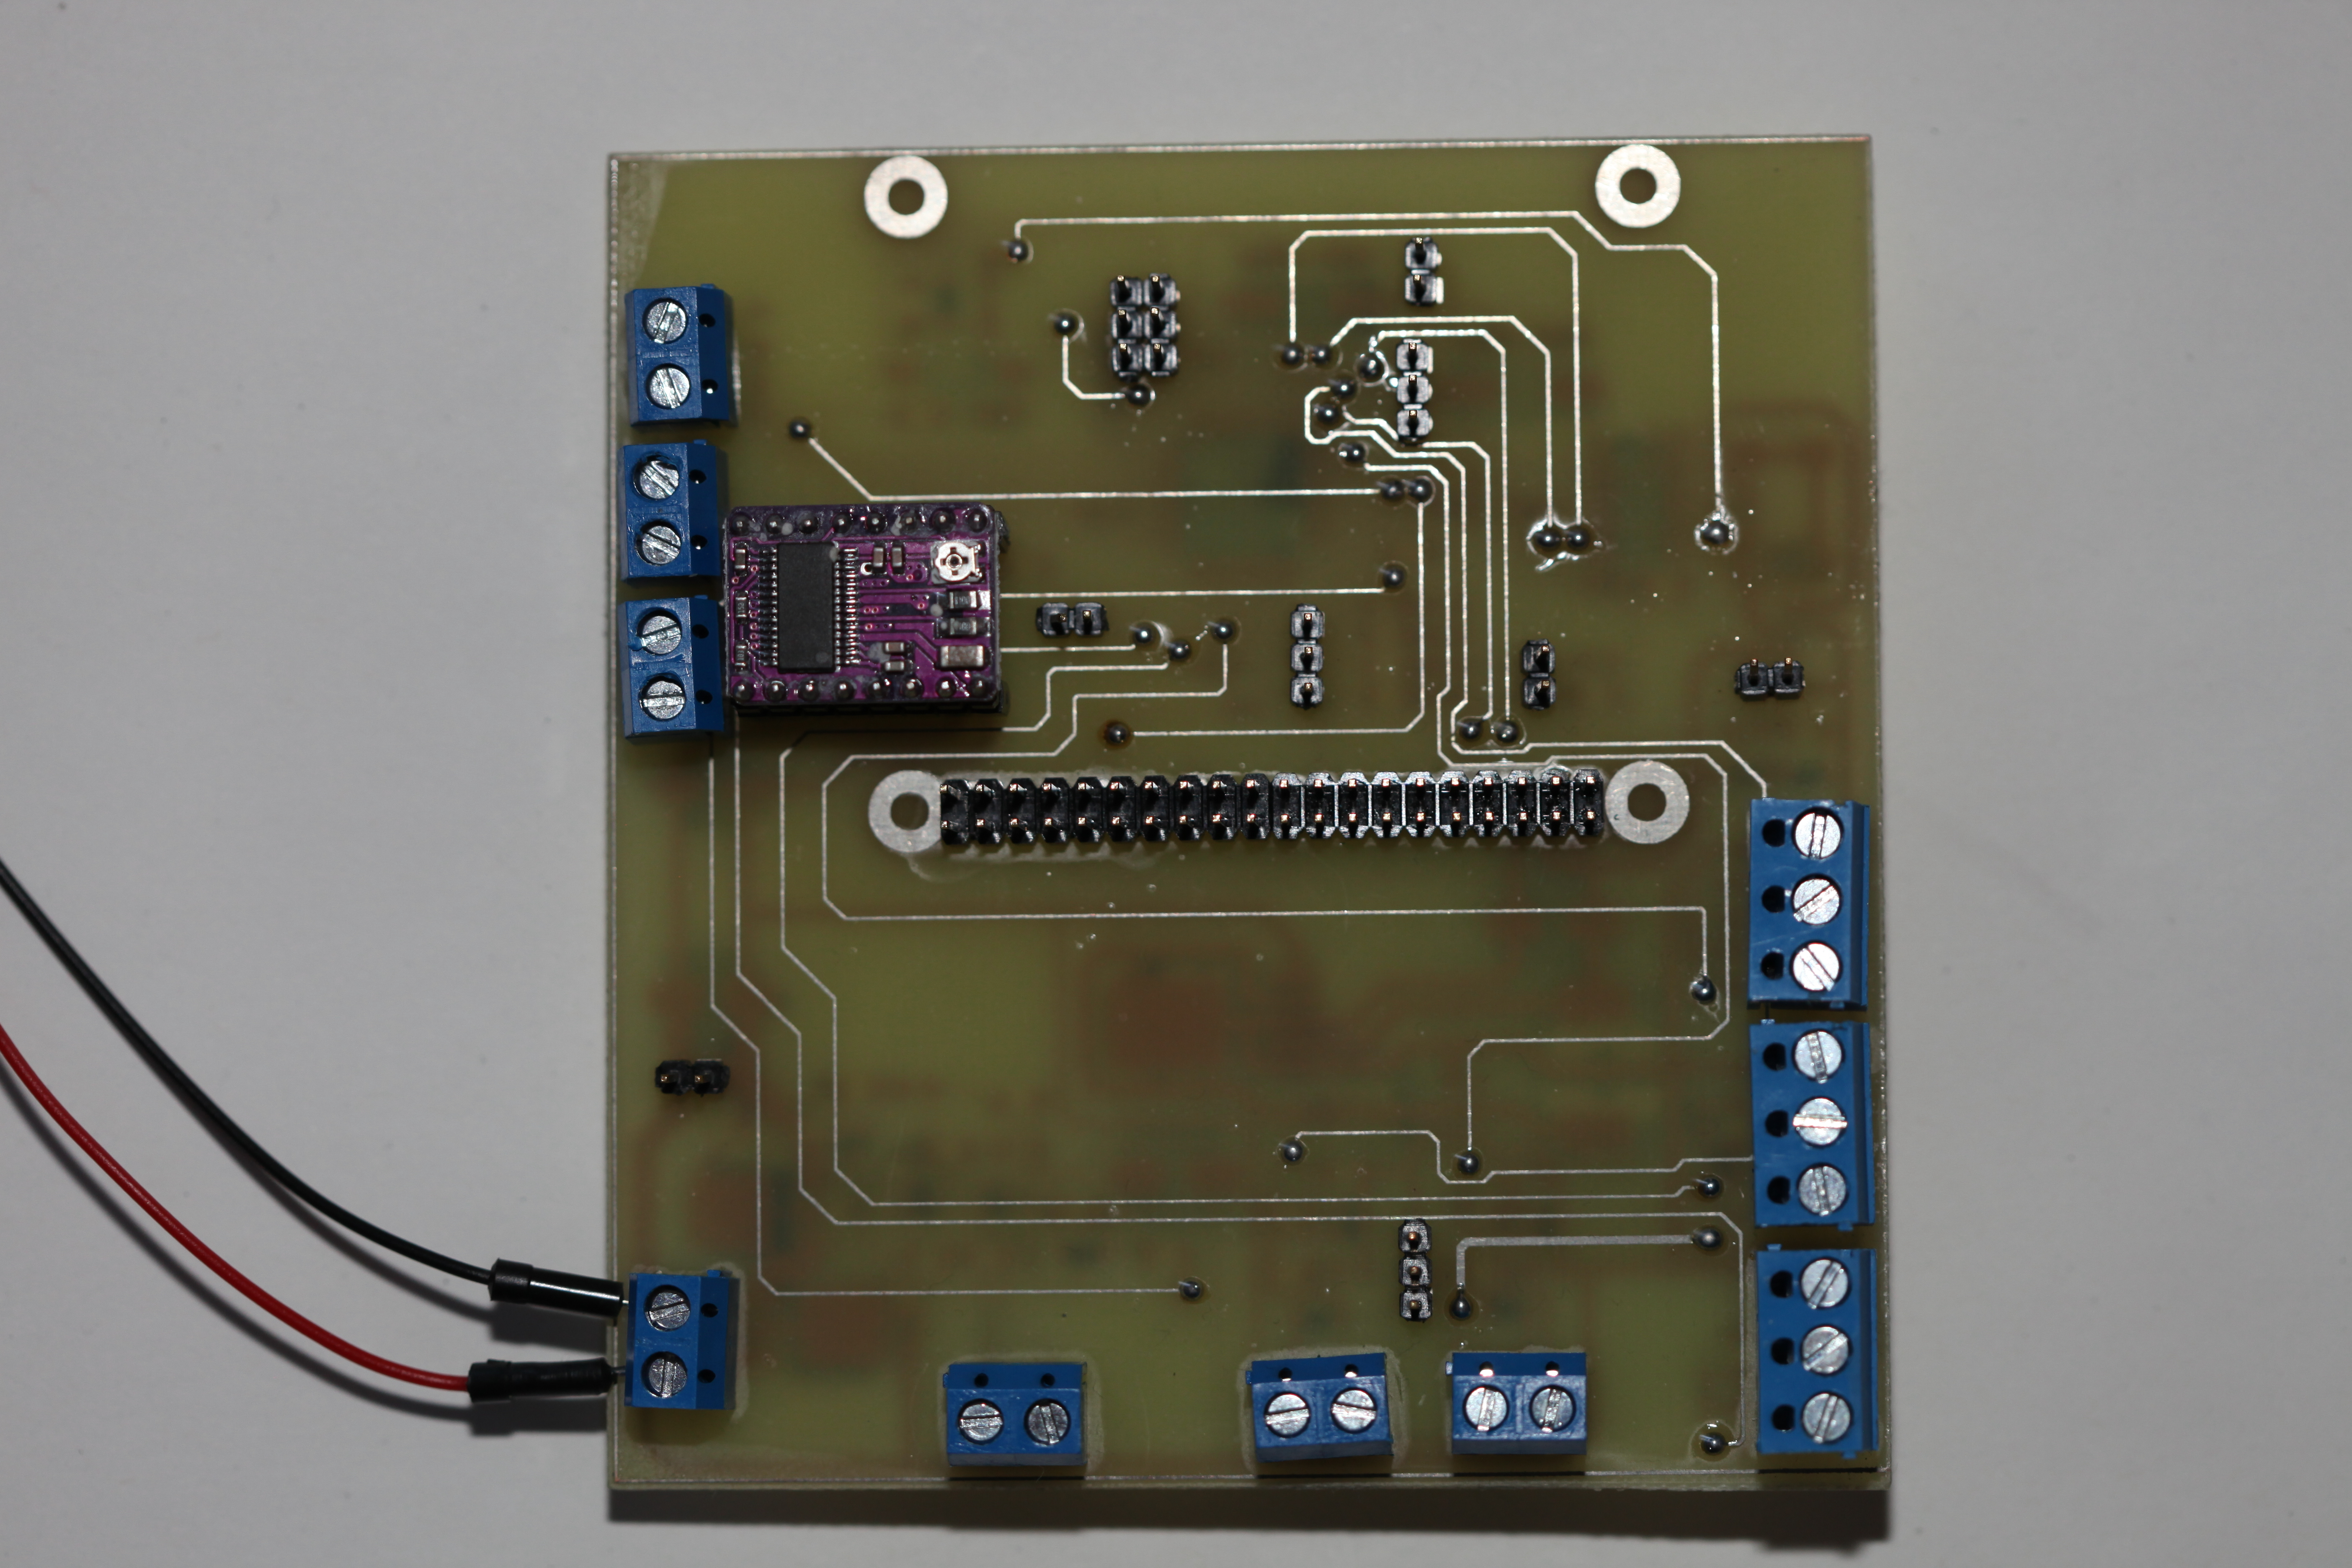
\includegraphics[scale=0.06]{fig/elektro/PrototypTop.jpg}
    \caption{Draufsicht der Oberseite}
\end{figure}

\begin{figure}[hb]
    \centering
    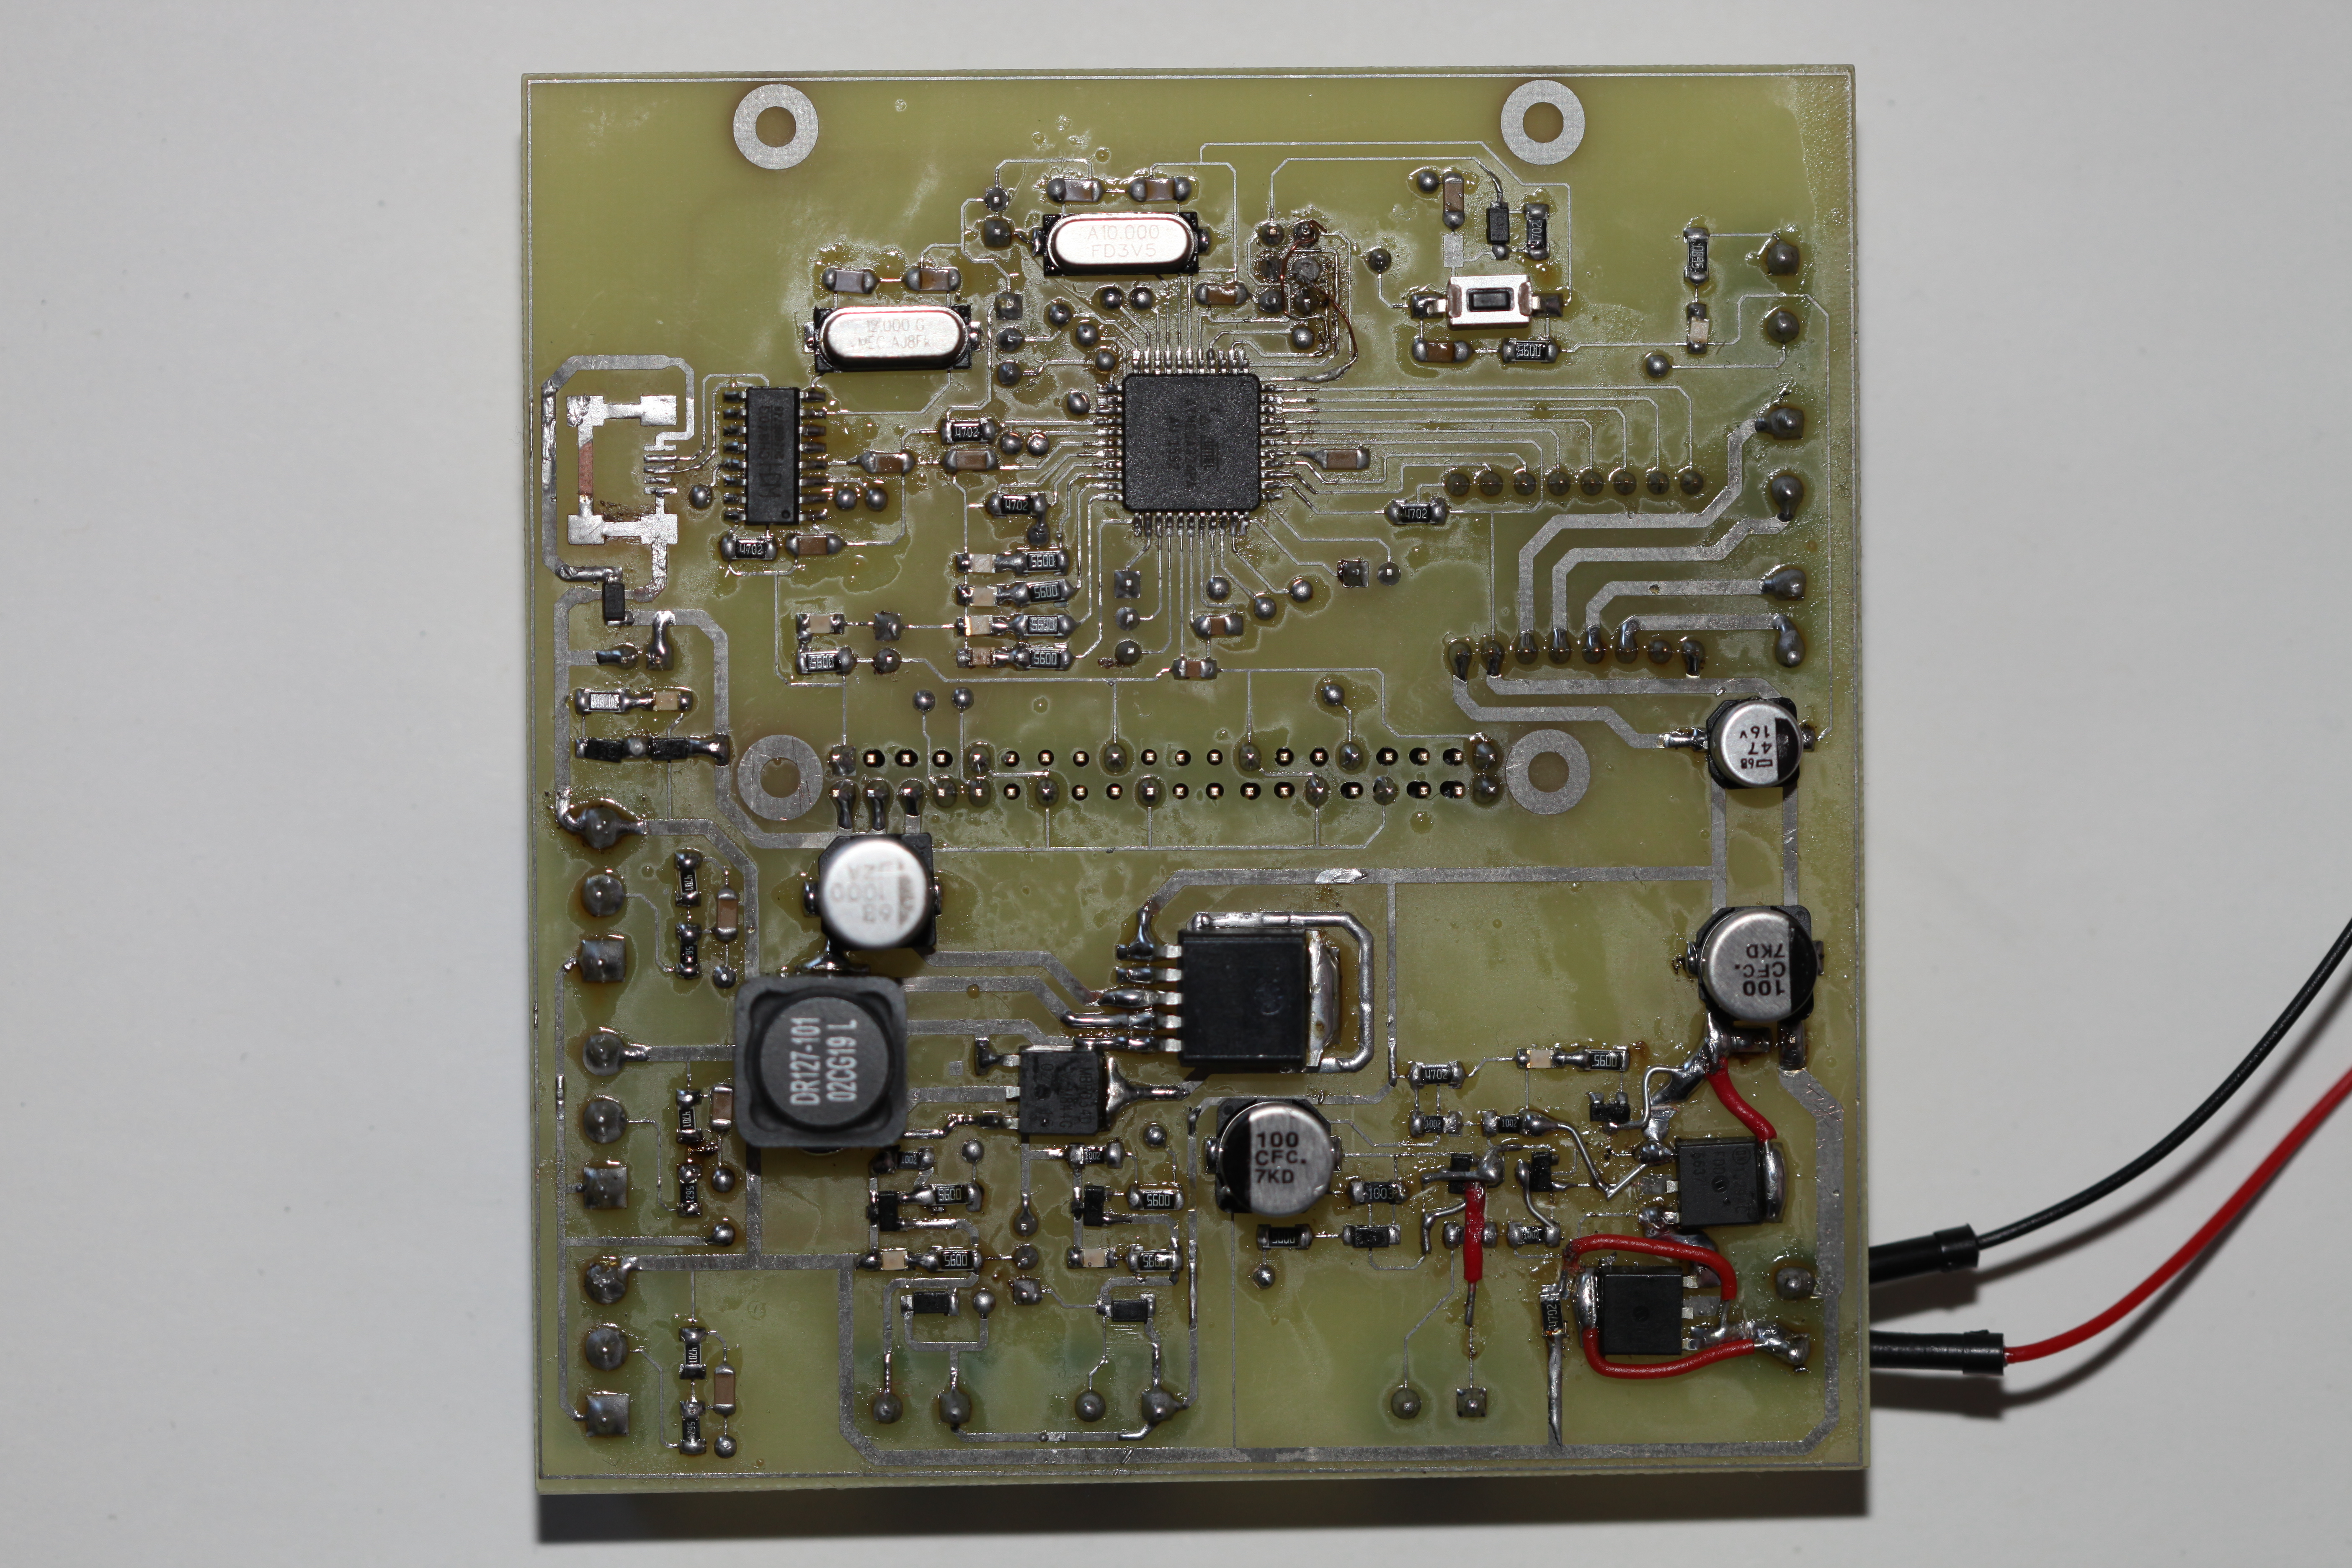
\includegraphics[scale=0.06]{fig/elektro/PrototypBot.jpg}
    \caption{Draufsicht der Unterseite}
\end{figure}

%/\-/\-/\-/\-/\-/\-/\-/\-/\-/\-/\-/\-/\-/\-/\-/\-/\-/\-/\-/\-/\-/\-/\-/\-/\-/\-/\-/\-/\-/\-/\-/\-/\-/\-/\-/\-/\-/\-/\-/\-/\-/\-/\-/\-/\-/\-/\-/\-/\-/\-/\-/\-/\-/\-/\-/\-/\-/\-/\-/\

\newpage
\section{Verbesserungsmöglichkeiten und Conclusio}
\subsection{Verbesserungsmöglichkeiten}

\subsubsection{Crowbar Circuit}
Sollte man die Versorgung des Raspberry Pi's über die Expansion Header Pins vornehmen, ist ein Überspannungsschutz nicht gegeben.
Eine essenzielle Schutzmaßnahme, um den Raspberry Pi bei einer zugeführten Überspannung nicht zu beschädigen, wäre eine sogenannte Klemmschaltung (engl.Crowbar Circuit).
Diese Art von Schaltung ermöglicht es, empfindliche Komponenten vor Überspannung zu schützen.

\begin{figure}[hpt]
    \centering
    \begin{circuitikz}[european, scale = 1.2]
        \draw (0,0) node[anchor=east] {-} to [short, o-*] (2,0);
        \draw (2,0) to [R,l=$R1$, *-*](2,2) to [/tikz/circuitikz/bipoles/length=1cm, zD-, l=$D1$,-*](2,4);
        \draw (2,2) to (3.5,2);
        \draw (2.8,2) to [C, l=$C1$, *-*](2.8,0);
        \draw (4,4) to [/tikz/circuitikz/bipoles/length=1.1cm, Ty-, mirror, l=$T1$,*-](4,0.915) to [short,-*](4,0);
        \draw (2,4) to [short, -o](0,4)node[anchor=east]{+};
        \draw (2,4) to [short, -o](6,4)node[anchor=west]{+};
        \draw (3,0) to [short, -o](6,0)node[anchor=west]{-};
        \draw (3,0) to (2,0) node[rground]{};
        \draw (0,3.8) -- node[left] {$U_\mathrm{e}$}node[sloped,currarrow,pos=1] {}(0,0.2);
        \draw (6,3.8) -- node[right] {$U_\mathrm{Last}$}node[sloped,currarrow,pos=1] {}(6,0.2);
    \end{circuitikz}
    \caption{Crowbar Circuit}
\end{figure}

\footfullcite{@TheArtOfElectronics-Kapitel-9.13.1-OvervoltageCrowbars}Bei einer zulässigen Versorgungsspannung gelangt die Zenerdiode nicht in einen leitenden Zustand und eine sichere Versorgung der dahinter liegenden Schaltung ist gegeben.
Der \acs{SCR} wird leitend, sobald der Wert der Versorgungsspannung jenen nominalen Zenerspannungswert der Zenerdiode und die Gate-Triggerspannung des Thyristors übersteigt.
Der Thyristor bleibt so lange im leitenden Zustand, bis dessen Anodenstrom unter wenige Milliampere fällt.
Ein niederohmiger Widerstand wird verwendet, um einen ausreichend hohen Zenerstrom zu generieren und um den SCR zu zünden.
Der Kondensator hat die Funktion, die Aktivierung der Crowbar-Schaltung durch harmlose Spannungsspitzen zu negieren.

Diese Schaltung konkret auf unsere Anwendung nutzbar gemacht, wären die Komponenten wie folgt zu wählen:
\begin{itemize}
    \item R1 mit 68Ohm
    \item D1 mit einer nom.Zenerspannung von 5.6V
    \item C1 mit 10nF
    \item T1 als TS1220-600B
\end{itemize}

Jene Schaltung hätte auch Nachteile, welche besonders die Wahl der Zenerdiode betreffen.
Zenerdioden sind nur in diskreten Werten mit bestimmten Toleranzen erhältlich.
Zusätzliche Toleranzen von etwa 5 Prozent bringt die 5V Versorgung über den LM2576-5 mit sich, welches somit einen Crowbar Circuit von mindestens 5.5V erfordert.
Dieses Minimum ist jedoch aufgrund von einem vorrübergehenden Überschwingen der geregelten Versorgung zu erhöhen:
Bei plötzlichen, großen Stromänderungen werden Spannungsspitzen erzeugt, welchen einige Wellen folgen.
Induktive Lasten, wie das Ventil oder die Pumpe, verschärfen dieses Problem aufgrund von remote sensing zusätzlich.
Die resultierenden Schwingungen führen zu Störungen in der Versorgung, welche die Crowbar-Schaltung jedoch nicht auslösen sollen.
Aus diesen Gründen sollte die Crowbar-Auslösespannung nicht unter 6V gewählt werden, jedoch sollte sie auch nicht über 7V gewählt werden,
da ansonsten das Risko der Zerstörung der Logikschaltungen gegeben wäre.
Rechnet man alle Toleranzen der Komponenten zusammen, ergibt sich eine Crowbar-Threshold-Voltage von etwa 5.9V bis 6.6V .

\subsubsection{Zusätzliche Beschaltung der Mikroprozessor-Anschlüsse}

Um hochfrequente Störimpulse auf Signal- und Versorgungsebene zu dämpfen sowie zusätzlichen Überspannungsschutz zu gewährleisten,
wäre folgende Implementierung, wie in der Automatisierungstechnik üblich, an jedem I/O-Pin des µC anzubringen.

\begin{figure}[htp]
    \centering
    \begin{circuitikz}[european, scale = 1]
        \draw (5,3) to [/tikz/circuitikz/bipoles/length=1.1cm, D-, l_=$D1$](5,6) to (5,6)node[vcc]{};
        \draw (2,0) to [short, -*](1,0) node[rground]{};
        \draw (8.5,0) to (8.5,0) node[rground]{};
        \draw (0,3) [short, o-] to (0.5,3);
        \draw (0.5,3) to [european inductor, l=$Ferrit$](2,3);
        \draw (2,3) to [R, l=$R1$](4,3) to [short, -*](4,3) to [short, -*](5,3);
        \draw (4,3) to [C, l_=$C1$, -*](4,0);
        \draw (5,0) to [/tikz/circuitikz/bipoles/length=1.1cm, D-, l_=$D2$,](5,3);
        \draw (5,3) to [R, l=$R2$](7,3);
        \draw (10,0) to (7,0) to (7,5) to (10,5) to (10,0);
        \draw (8.5,3)node[anchor=north]{µC};
        \draw (0,2.7) -- node[left] {$U$}node[sloped,currarrow,pos=1] {}(0,0.3);
        \draw (0,0) to [short, o-](5,0);
        \draw (8.5,5) to (8.5,6)node[vcc]{};
    \end{circuitikz}
    \caption{Beschaltung der I/O-Pins des µC}
\end{figure}

\newpage

\subsection{Zusammenfassung}

Das Ziel dieser Arbeit war, eine elektronische Steuereinheit zu kreieren, welche in der Lage ist, jegliche Aktoren anzusteuern, Sensoren einzulesen und mit einem Raspberry Pi Information auszutauschen.
Eingehende Information soll über den vorgesehenen Mikrocontroller verarbeitet, und Prozesse über diesen ausgeführt werden. \\

Mit diesen Anforderungen wurde ein Schaltplan erstellt und eine Platine geplant, entworfen, gefertigt und bestückt.
Durch ausführliches Testen wurden Fehlerquellen und einzelne Mängel korrigiert, sodass ein funktionstüchtiger Prototyp zu Stande kam.\\

\subsection{Conclusio}

Nach Ansicht des Autors hat dieser viel Wissen in den Bereichen Projektorganisation, Prototyping und Hardwaredesign erlangt.
Das durch diese Arbeit erworbene Fachwissen in verschiedenen Softwareprodukten,
in Schaltungsdimensionierungen allgemein sowie in der Praxis gemachte Fehler erachtet der Autor als essenziell und wegweisend für die Zukunft.

%/\-/\-/\-/\-/\-/\-/\-/\-/\-/\-/\-/\-/\-/\-/\-/\-/\-/\-/\-/\-/\-/\-/\-/\-/\-/\-/\-/\-/\-/\-/\-/\-/\-/\-/\-/\-/\-/\-/\-/\-/\-/\-/\-/\-/\-/\-/\-/\-/\-/\-/\-/\-/\-/\-/\-/\-/\-/\-/\-/\
